\chapter{Implementace}

V předchozí kapitole jsme navrhli strukturu, které se náš projekt bude držet. Stejně tak již víme, jakým způsobem bude se systémem interagovat hráč. Nyní můžeme přistoupit k jeho implementaci.

V této kapitole zběžně představíme, jak jsme celkově při implementaci postupovali, zevrubněji pak vylíčíme, jak jsme přistupovali k řešení překážek, které nám postavil do cesty zejména fyzikální subsystém. 

Podrobnou programátorskou dokumentaci k jednotlivým komponentám psanou v anglickém jazyce lze nalézt v příloze. Zvolili jsme pro ni standardní formát dokumentačních komentářů exportovaných do souboru XML, protože ten podporuje pohodlnou integraci s IDE (např. použití v našeptávači).

\subsubsection*{Závislosti}
Naše řešení používá několik externích knihoven. Pro procedurální animaci šermířova modelu jsme využili balíček AnimationRigging \cite{AnimationRigging}. S tvorbou dalších kosmetických efektů vypomohla knihovna DOTween \cite{DoTween}. Dále Math.NET Numerics \cite{MathDotNetNumerics} poskytlo stabilní a dobře testovaný nástroj pro řešení soustav lineárních rovnic. Newtonsoft.Json \cite{NewtonsoftJson} jsme použili k serializaci do formátu JSON. TextMesh Pro \cite{TextMeshPro} pomohlo při tvorbě prvků GUI. Repozitoř SubclassPropertyDrawer \cite{SubclassPropertyDrawer} umožnila pohodlnou editaci jednotlivých SwordMovement.Modules v editoru. 

Dále je třeba poděkovat uživatelům unity fóra \cite{InvertReverseUIMask}, které pomohlo s implementací grafické reprezentace healthbaru.

Největší díky však patří github uživateli \textit{mstevenson}, jehož práce \cite{ConfigurableJointExtensions} citelně pomohla s použitím cílové rotace na jointech - bez kterého by implementace zásadní části této práce nebyla možná.


\section{Implementace základních komponent}

Objektový návrh základních entit našeho systému již známe z předchozí kapitoly. Zde si podrobně nastíníme implementaci \textbf{šermíře} a jeho \textbf{meče} - nejprve vnitřní implementaci šermíře, potom meče, následně kosmetickou stránku šermíře (ta operuje víceméně odděleně od jeho základního fungování) a nakonec toto vše protkáme damage systémem. 

Vynecháme algoritmy jednotlivých modulů ovládání - ty jsme již podrobně nastínili v \ref{interfacesSwordMovementModulesSubsection} - a rovněž pro objekt kořenu hierarchie je implementace natolik přímočará, že se jím zde nebudeme zaobírat. 


\begin{figure}[p]\centering
  \center
  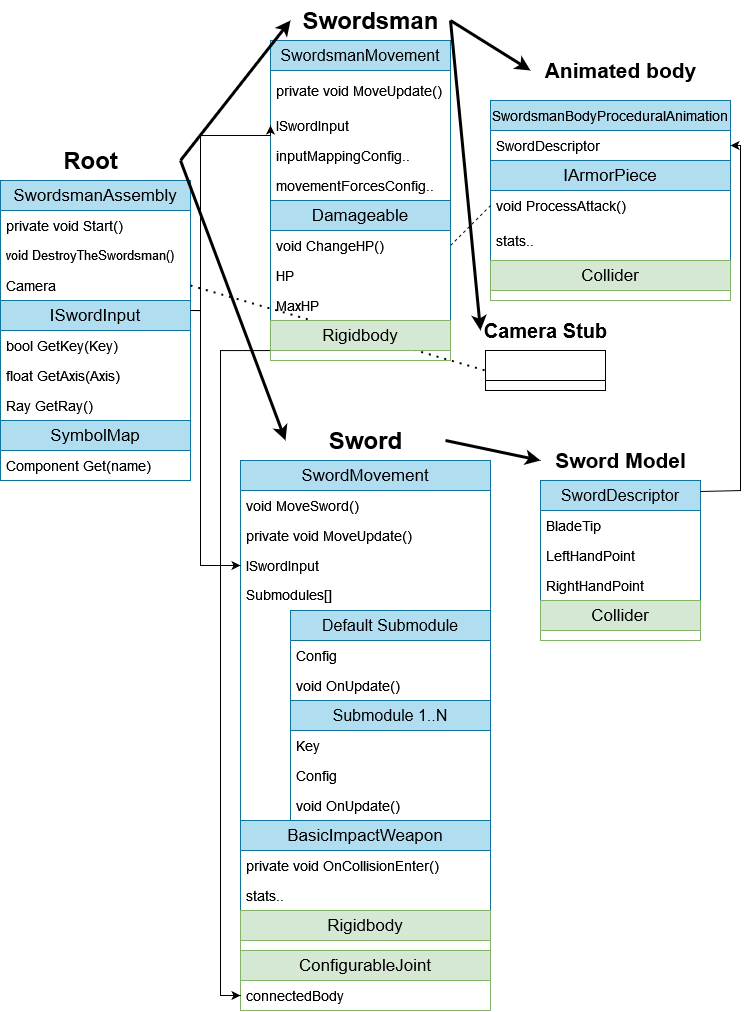
\includegraphics[width=145mm]{../img/Structure-diagram-impl.png}
  \caption{Diagram znázorňující strukturu našeho systému - modře vlastní komponenty, zeleně vestavěné}
  \label{obr05:objectModelDiagramReprise}
\end{figure} 
 
\pagebreak

%------------------------------------------------------------------------------------------------------------------------------------------------------------------------------------------------------------------------------------------------------------%
 % xxxxxxxxxxxxxxxxxxxxxxxxxxxxxxxxxxxxxxxxxxxxxxxxxxxxxxxxxxxxxxxxxxxxxxxxxxxxxxxxxxxxxxxxxxxxxxxxxxxxxxxxxxxxxxxxxxxxxxxxxxxxxxxxxxxxxxxxxxxxxxxxxxxxxxxxxxxxxxxxxxxxxxxxxxxxxxxxxxxxxxxxxxxxxxxxxxxxxxxxxxxxxxxxxxxxxxxxxxxxxxxxxxxxxxxxxxxxxxxxxxxxxxxx %
%------------------------------------------------------------------------------------------------------------------------------------------------------------------------------------------------------------------------------------------------------------%


\subsection{Šermíř}

Šermíř je herní objekt, který reprezentuje hráče v herním světě. Potřebujeme od něj, aby byl schopen se pohybovat po herním světě a umožnil hráči skrze své oči nahlížet na svět. 

Instrukce od hráče bude přijímat z přidělené instance \textit{ISwordInput}.

\subsubsection*{Pohyb}

Zásadním rozhodnutím, které jsme učinili, bylo implementovat šermíře jako \textbf{nekinematické Rigidbody}, ovládané čistě skrze fyzikální systém působením sil. 

\textit{Nejde o standardní postup - typicky je ve hrách pohyb postavy řešen přímo ze skriptu upravováním její polohy, postava může působit silami na okolní předměty, ale ne obráceně. Důvody jsou zřejmé - tvůrci hry takto získají větší kontrolu, která jim umožní ručně ladit pohyb postavy pro optimální hráčský zážitek; dále je často výslovně nevhodné, aby na hráčskou postavu působily silami okolní kolidující předměty - především při pohledu z 1. osoby, kdy hráč o převážně části svého těla nemá přehled (nezpozorovaná kolize, která postavu odmrští, pak může působit dojmem glitche). Unity pro tento standardní přístup poskytuje vyladěnou komponentu CharacterController.}

\textit{Pohyb hráče skrze fyzikální systém jsme zvolili zkrátka proto, že se zdál jako zajímavá oblast hodná prozkoumání. Přináší netriviální výzvy v oblasti zaručení stability hráčské postavy a responzivity ovládání. Na druhou stranu má šanci nám poskytnout další element navíc k meči, který může umocnit hráčovy možnosti fyzikální interakce s okolním prostředím\footnote{Např. s jeho přítomností můžeme zadarmo implementovat jednoduché fyzikální hádanky ala vyvažovací lávka v 2.misi Half-Life 2 \cite{HalfLife2}} a s nepřátelským mečem.}

Jak jsme tedy postupovali? Do herního objektu odpovídajícího hráči jsme umístili komponentu Rigidbody. Váhu jsme nastavil na 60 - cca odpovídající pro typického člověka, jinak jsme ponechali výchozí hodnoty. Pro účely kolizí s herním prostředím jsme do potomka umístili jednoduchý CapsuleCollider se standardně používanými rozměry 2 x 0.5. Kapsle do sebe zhruba obsáhne šermířův model, ale nemá žádné ostré hrany, o které by se šermíř mohl zadrhávat při pohybu členitým terénem. Kolizní vrstvy jsme nastavili tak, aby tato kapsle kolidovala s terénem, ale ne s nepřáteli ani jejich zbraněmi.

Takto tedy vypadá fyzikální reprezentace šermíře, nyní k jejímu ovládání. Pro to jsme již určili zodpovědnou komponentu \textbf{SwordsmanMovement}. 

Konkrétní metody pohybu, které podporuje, jsou:
\begin{itemize}
  \item \textbf{Chůze dopředu/dozadu} - lineární posun dopředu o kladnou nebo zápornou vzdálenost
  \item \textbf{Úkrok doleva/doprava} - lineární posun doprava o kladnou nebo zápornou vzdálenost
  \item \textbf{Natočení se doleva/doprava} - rotace kolem šermířovy vertikální osy o kladný nebo záporný úhel, mění význam \textit{dopředu} a \textit{doprava}
  \item \textbf{Skákání} - okamžité aplikování impulzu na tělo hráče, pouze pokud hráč stojí na zemi
\end{itemize}

Pro každou z těchto akcí komponenta umožňuje nakonfigurovat vstupní osu, ze které budou funkcí \textit{ISwordInput.GetAxis()} čteny instrukce (čísla v intervalu [-1;1]), dále rovněž číslo udávající rychlost pohybu. Pro skok je konfigurována aktivační klávesa a vektor síly impulzu.

\subsubsection*{Pohyb - Lineární pohyb}

Naivním přístupem k pohybu hráče by bylo zkrátka každý FixedUpdate přečíst hodnotu na příslušné ose, tu vynásobit s rychlostí, z této finální rychlosti získat sílu (nazvěme ji \textit{targetMovement}) vynásobením s vektorem udávajícím směr (dopředu/doprava), a tu aplikovat pomocí \textit{rigidbody.AddForce()}.
Tento přístup hráčem skutečně pohybuje ve správném směru, ne však způsobem, jaký bychom chtěli. Každá změna pohybu má pomalý rozjezd a jakmile se rozjede, dostat se z ní zpátky trvá stejně dlouho. Dlouhodobým pohybem v jednom směru šermíř stále zrychluje (hranicí je až rychlost světla). Rovněž se šermíř nijak nesnaží odolávat kolizím, které na něj působí. 

Řešením je vypočítanou hodnotu \textit{targetMovement} neinterpretovat jako sílu, ale jako cílovou rychlost šermíře. Aktuální rychlost šermíře lze získat jako \textit{rigidbody.velocity}. Spočítáme tedy \textit{targetMovement}s v jednotlivých směrech a sečteme je dohromady. Takto aplikujeme sílu, která šermíře dostane na požadovanou rychlost. 

\begin{code}
 var velocityDelta = targetMovement - rigidbody.velocity;
 rigidbody.AddForce(velocityDelta, ForceMode.VelocityChange);
\end{code}


Takto se šermíř pohybuje responzivně (téměř okamžitě dosáhne požadované rychlosti, i při změně směru) a není mu umožněno nekontrolovaně zrychlovat. Pohyb působí plynulým dojmem díky tomu, že náš vstup - \textit{ISwordInput.GetAxis()} - zaručuje\footnote{Analogicky jako \textit{UnityEngine.Input.GetAxis()}.} postupný plynulý náběh a změnu hodnoty.

Interně bude síla šermíři aplikována v průběhu nadcházejícího kroku fyzikální simulace, v platnost tedy vstoupí snímek následující po její aplikaci. Další síly, které na objekt působí, při výpočtu nejsou brány v úvahu, ty tedy stále jsou schopny na objekt působit a z naší cílové rychlosti ho vychýlit - objekt tedy velmi důrazně vybízíme, aby přešel na danou rychlost, stále však reaguje na ostatní síly. 

Celková odolnost proti jednorázovým kolizím je však (v horizontálním směru) velmi značná - ať už kolize na objekt vyvine jakoukoliv sílu, nejpozději v průběhu několika dalších snímků po ukončení jejího působení bude plně vstřebána. Pokud bychom chtěli odolnost omezit, nic nám nebrání stanovit ještě číslený parametr (\textit{maxChange}), kterým bude omezena maximální velikost síly, kterou v jednom snímku působíme - zhruba takto:

\begin{code}
 var velocityDelta = targetMovement - rigidbody.velocity;
 var deltaMagnitude = Mathf.Min(velocityDelta.magnitude, maxChange);
 velocityDelta = velocityDelta.normalized * deltaMagnitude;
\end{code}

Takto omezíme maximální sílu, kterou může v jednom snímku šermíř vyvinout na vstřebání kolize - kolize tedy stále bude vstřebána, avšak potrvá to déle.

Kombinací všech těchto faktorů docházíme k mixu, který není o mnoho méně hráčsky přívětivý, než tradiční pohyb přímým přepisováním pozice. Jako bonus je šermíř stále schopen být ovlivňován kolizemi s ostatními předměty, avšak míru, do které mu to je umožněno, máme pod kontrolou.

\subsubsection*{Pohyb - Rotační pohyb}
Rotaci šermíře kolem jeho osy implementujeme analogicky. Nejprve spočítáme \textit{targetAngularMovement} jako rotaci kolem vertikální osy šermíře o úhel získaný z \textit{ISwordInput.GetAxis()} násobeno rychlost. Rotační pohyb následně vykonáme takto:

\begin{code}
 var angularVelocityDelta = 
     targetAngularMovement - rigidbody.angularVelocity;
 rigidbody.AddTorque(angularVelocityDelta, ForceMode.VelocityChange);
\end{code}

Je zde však třeba vyřešit ještě jeden problém - \textbf{klácení postavy na stranu}. 

Typicky se očekává, že šermíř stojí v dokonale vzpřímené pozici. Jakékoliv i jen velmi drobné, ale dlouhodobější vychýlení herní kamery ze svislého pohledu (jiné než kontrolovaný efekt třesení kamerou) na hráče typicky působí nežádaným zneklidňujícím až matoucím dojmem. Odchýlením vertikální osy hráče od globální osy Y se rovněž náš předchozí představený systém pro lineární pohyb dostane do neočekávaného stavu. 

Při fyzikální kolizi je však vyvolání rotace napříč všemi 3 stupni volnosti typickým chováním. Jak tedy spolehlivě zařídíme, aby bylo možné rotovat šermíře pouze kolem jeho vertikální osy?

Přímočarým řešením, které se nabízí, jsou flagy \textit{rigidbody.constraints}, jež nalezneme přímo na šermířově komponentě Rigidbody a hlásají, že přesně náš požadavek umožňují splnit. Jednoduše tedy zaškrtneme pole \textit{FreezeRotationX} a \textit{FreezeRotationZ}. Spustíme hru a řešení se tváří fungovat. Jak se šermíř pohybuje po členitém terénu, pozorujeme však, že se na něm stále nějaký náklon hromadí - velmi pomalu, ale znatelně.

Důvod tohoto chování najdeme v \href{https://docs.unity3d.com/2022.2/Documentation/ScriptReference/Rigidbody-inertiaTensor.html}{oficielní dokumentaci} \cite{Unity} - dle té jsou specificky rotační constraints implementovány pouze přepsáním hodnot jiné komponenty - \textit{rigidbody.inertiaTensor}. Ta zjednodušeně řečeno udává, jak obtížná je pro daný útvar rotace v jednotlivých stupních volnosti. Její nastavení je vyhodnocováno jako jeden ze vstupů pro constraint solver. Tedy i pokud nastavíme obtížnost v daném stupni volnosti na nekonečno (jako to rigidbody.constraints dělá), numerická nepřesnost constraint solveru (viz \ref{physicsIntroSimulationStabilitySubsection}) zkrátka drobným změnám umožní, aby se proplížily.

Řešením, které funguje, je navíc k uzamčení os X a Z přidat ještě kus herní logiky, který každý snímek rotaci v obou osách ručně vynuluje.

\subsubsection*{Pohyb - Skákání}

Vykonání skoku je jednoduché - zkrátka pokud byla stisknuta příslušná klávesa a šermíř stojí na zemi, dodáme šermířovi nakonfigurovaný impuls - nějak takto:

\begin{code}
 rigidbody.AddForce(jumpForce, ForceMode.Impulse);
\end{code}

Netriviální částí je rozhodnout, zda \textbf{šermíř stojí na zemi}. K tomuto účelu jsme umístili v oblasti jeho nohou podobjekt obsahující collider s flagem \textit{collider.isTrigger} nastaveným na true a nakonfigurovali jeho kolizní vrstvy, aby kolidoval pouze s terénem. Pokud tento collider aktuálně koliduje s dalším colliderem, který není trigger, chceme šermíře považovat za uzemněného. Unity však neposkytuje žádnou funkci, které bychom se mohli jednoduše zeptat, zda collider s něčím koliduje. 

Implementovali jsme tedy vlastní komponentu \textit{TriggerActivityInfo}, která poslouchá klasicky na zprávy \textit{OnTriggerEnter()} a \textit{OnTriggerExit()} a dle nich si manuálně vede záznamy o probíhajících kolizích. Umístili jsme ji do stejného objektu\footnote{Zde je důležité, že oba jsou ve stejném herním objektu, který je oddělený od Rigidbody - jinak by \textit{TriggerActivityInfo} buď nedostávalo žádné zprávy, nebo dostávalo od všech triggerů napříč šermířem - viz \ref{collidersPhysicsIntroSubsection}} jako náš triggercollider a toho se již \textit{SwordsmanMovement} může civilizovaně ptát, zda je aktuálně probíhajících kolizí více než nula.

\subsubsection*{Kamera}

Nyní je hráč schopen pohybu po herním světě, stále však zbývá zajistit, aby mohl svět \textbf{vizuálně vnímat}. K tomuto účelu nám Unity poskytuje objekt \textbf{kamery} - ta zkrátka definuje bod, ze kterého se scéna vykresluje na obrazovku. Natočení jejího \textit{Transformu} určuje natočení pohledu. Chtěli bychom tedy, aby se tato kamera nacházela na vhodném místě zhruba v oblasti šermířových očí. Také by bylo příhodné, aby hráč byl schopen kontrolovat její rotaci - rozhlížet se.

Řešení je jednoduché - kameru jsme umístili v objektové hierarchii mezi děti šermířova herního objektu, napolohovali jsme ji na příhodné místo u jeho očí, a nyní se při šermířově pohybu přesunuje adekvátně spolu s ním. 

Dále chceme hráči umožnit rozhlížení se - to znamená měnit rotaci kamery v jejích osách X a Y. Obdobně jako u pohybu, zde rovněž pro každou osu rotace nabídneme uživateli, aby nakonfiguroval osu vstupu a rychlost. Následně voláním\textit{ ISwordInput.GetAxis()}, vynásobením výsledku s rychlostí a s \textit{Time.deltaTime}\footnote{Pohyb kamery je kosmetickou záležitostí, která nijak nesouvisí s fyzikou - narozdíl od pohybu šermíře jej tedy nevykonáváme z FixedUpdate, ale z Update.} získáme úhel, který jednoduše přičteme k eulerovské reprezentaci rotace na \textit{Transformu} kamery\footnote{V praxi její eulerovský úhel nečteme v každém snímku znovu - přečteme ho jednou při inicializaci a tuto jeho verzi ''nakešovanou'' jako 3D vektor následně považujeme za zdroj pravdy - doporučený postup dle \href{https://docs.unity3d.com/2022.2/Documentation/ScriptReference/Quaternion-eulerAngles.html}{\underline{oficielní dokumentace}} \cite{Unity}}. Aby rozhlížení nebylo až příliš volné, pro každou osu ještě přidáme z editoru konfigurovaný minimální a maximální úhel.

\textit{Na horzizontální a vertikální osu rozhlížení jsme přiřadili vstup z horizontální a vertikální osy pohybu myši. Po herním testování jsme však došli k závěru, že rozhlížení do stran je velmi matoucí a znepřijemňuje ovládání meče. V praxi je tedy rychlost horizontálního rozhlížení nastavena na 0. Rozhlížení nahoru/dolů pomocí vertikální osy myši jsme ponechali - zdá se být použitelné bez větších problémů.}

Pohyb kamery se zdá přijatelně funkční, dopustili jsme se však prohřešku proti štábní kultuře. Kamera je velmi důležitým singletonem z hlediska scény a není vhodné, aby byla schována uvnitř šermířovy hierarchie. V budoucnu chceme mít ve hře šermířů více a není možné, aby měl kameru každý z nich. Navíc došlo-li by k šermířově smrti, kamera by jakožto jedno z jeho dětí byla zničena rovněž - tím by se celý herní systém mohl dostat do nedefinovaného stavu.

Pro řešení si povšimněme, že jediné, co na kameře využíváme, je její \textit{Transform}. Stačí ji tedy uvnitř šermíře nahradit obyčejným prázdným herním objektem - šermířova logika nepozná rozdíl. Skutečnou kameru ponecháme jako samostatný objekt ve scéně, vybavený komponentou (\textit{CameraFollowPoint}), ve které je nakonfigurovaný odkaz na tento prázdný herní objekt v jednom konkrétním šermířovi\footnote{Za jeho konfiguraci je zodpovědná šermířova komponenta SwordsmanAssembly.}. Tato komponenta jednoduše těsně před vykreslením každého snímku\footnote{K tomu slouží standardní zpráva LateUpdate().} změní světovou pozici a rotaci \textit{Transformu} kamery, aby odpovídala světovým souřadnicím onoho cílového objektu. 

\subsubsection*{Shrnutí}

Šermíř se pohybuje po světě a ovládá kameru, skrze kterou hráč vidí svět. Jeho pohyb po světě probíhá čistě skrze fyzikální systém působením sil - tedy netradiční metodou, ale podařilo se nám dobrat k implementaci, která umožňuje velmi přijatelnou responzivitu a pohodlnost ovládání. 

Neméně důležitá je však stránka kosmetická - šermířův 3D model a animace, pomocí kterých drží meč. K tomu, abychom si je mohli představit, však nejprve potřebujeme znát implementaci meče. 


%------------------------------------------------------------------------------------------------------------------------------------------------------------------------------------------------------------------------------------------------------------%
 % xxxxxxxxxxxxxxxxxxxxxxxxxxxxxxxxxxxxxxxxxxxxxxxxxxxxxxxxxxxxxxxxxxxxxxxxxxxxxxxxxxxxxxxxxxxxxxxxxxxxxxxxxxxxxxxxxxxxxxxxxxxxxxxxxxxxxxxxxxxxxxxxxxxxxxxxxxxxxxxxxxxxxxxxxxxxxxxxxxxxxxxxxxxxxxxxxxxxxxxxxxxxxxxxxxxxxxxxxxxxxxxxxxxxxxxxxxxxxxxxxxxxxxxx %
%------------------------------------------------------------------------------------------------------------------------------------------------------------------------------------------------------------------------------------------------------------%




\subsection{Meč}

Meč je herní objekt, který slouží jako šermířův nástroj (násilné) interakce s okolím. Jedním z hlavních předsevzetí naší práce bylo implementovat ho jako objekt ovládaný plně skrze fyzikální systém - schopný působit silami na ostatní objekty a realisticky reagovat na síly, jež působí na něj.

Jeho chování by mělo odpovídat tomu, že je šermířem uchopen v nějakém dobře definovaném bodě svého těla - ideálně na rukojeti. Kolem tohoto bodu by mělo být možné meč libovolně rotovat ve všech třech stupních volnosti. Tři stupně volnosti by měly být umožněny i pro lineární pohyb celého meče spolu s jeho bodem úchopu v prostoru. Veškeré tyto změny své polohy by meč měl vykonávat realisticky plynule působením síly v průběhu času.

\subsubsection*{Model meče}

Nejprve jsme jako samostatný objekt vytvořili model meče. Grafickou reprezentaci jsme vymodelovali\footnote{Použití 3D modelu třetí strany by zkomplikovalo vydání našeho projektu pod opensource licencí.} v programu Blender \cite{Blender} - pro naše účely je důležité pouze to, že existuje. Kolem té jsme následně rozmístili collidery - jeden BoxCollider rovnoběžně s čepelí, vedoucí od špičky meče až po konec rukojeti; kolmo na něj druhý BoxCollider pro záštitu - viz obr.\ref{obr05:swordWithColliders}. 
\begin{figure}[ht]\centering
  \center
  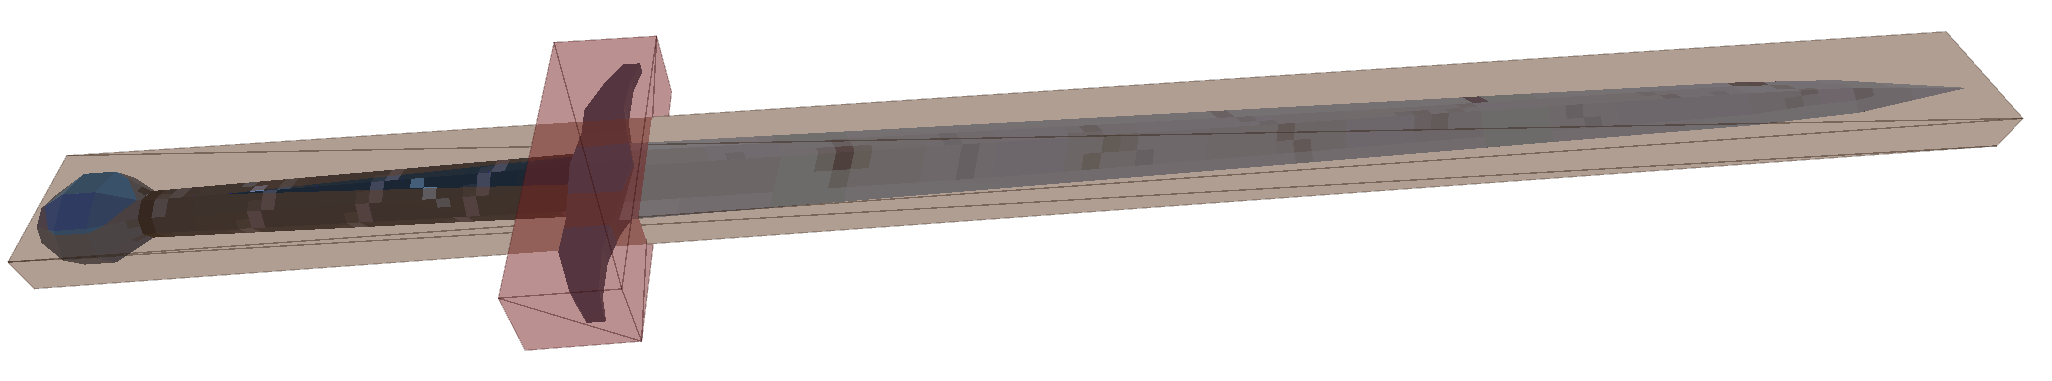
\includegraphics[width=120mm]{../img/swordWithColliders.png}
  \caption{Model meče s rozmístěnými collidery}
  \label{obr05:swordWithColliders}
\end{figure} 
Hoden povšimnutí je značný přesah, jenž jsme colliderům dopřáli - ten je v praxi pro hráče nezaznamenatelný, pouze meč činí méně náchylným na tunelování a obecné nestabilní chování, jež by nastávalo kdyby collidery těsně kopírovaly grafický model.  

Na mnoha místech herní logiky\footnote{Např. v modech pro ovládání meče (\ref{interfacesSwordMovementBlockingModuleSubsubsection}) nebo při korekci kolizí (\ref{swordCollisionsSection}).} se meč účastní geometrických výpočtů - v těch s ním typicky pracujeme jako s množinou několika pojmenovaných význačných bodů. Ty vyznačíme zde přímo na modelu meče. Každému z nich bude odpovídat jeden prázdný (pouze s komponentou \textit{Transform}) podobjekt našeho modelu. Abychom nemuseli úmorně přetahovat jednotlivé \textit{Transformy} v editoru na každé místo, kde provádíme výpočty, vytvořili jsme komponentu \textit{SwordDescriptor} - ta pro každý význačný bod definuje serializovatelnou proměnnou - stačí tedy každý bod v editoru přetáhnout pouze do této komponenty, cizím objektům dále budeme předávat odkaz na ní.

\bigbreak

Takto definovaný model meče je samostatně existenceschopnou entitou. Nic nám tedy nebrání vytvořit z něj vlastní prefab.

\subsubsection*{Základní struktura} 

Nyní přistupme k hlavnímu objektu meče. Do toho jsme umístili výše popsaný model meče jako dítě. Hlavní objekt je zodpovědný za účast meče ve fyzikální simulaci a za hráčovu schopnost meč ovládat.

Vstup od hráče přijímá, stejně jako šermíř, z komponenty \textit{ISwordInput}.

Najdeme zde dvě hlavní komponenty fyzikálního systému - nekinematické \textit{Rigidbody} a \textit{ConfigurableJoint}.

\textbf{Rigidbody} jsme stanovili váhu 1.5 (typická váha jedenapůlručního meče), později jsme došli k objevu, že pro optimální hráčský zážitek je třeba vypnout gravitaci a ručně nastavit těžiště a \textit{intertiaTensor} - o tom zevrubněji v \ref{swordParameterTweaksSection}.

\textbf{ConfigurableJoint} meči velmi přímočaře poskytl schopnost být držen šermířem - stačí nastavit šermířovo \textit{Rigidbody} jako \textit{connectedBody} jointu. \textit{Anchor} jsme umístili doprostřed rukojeti - to je bod, ve kterém šermíř meč ''drží''. 

Z objektového návrhu již známe komponentu \textbf{SwordMovement}, jejímž úkolem je řídit rigidbody a joint tak, aby se meč pohyboval způsobem odpovídajícím hráčskému vstupu.


\subsubsection*{Metoda MoveSword()} \label{swordMovementMoveSwordImplementationSubsection}

Z předchozí kapitoly bychom již měli být seznámeni se strukturou komponenty \textbf{SwordMovement}. Víme tedy, že hostuje množinu modulů - ty slouží jako zdroj high-level instrukcí udávajících cílovou polohu meče. Tyto instrukce jsou \textit{SwordMovement}u předávány voláním metody \textit{MoveSword()}.

Této metodě je typicky předána nová pozice, od té předchozí libovolně vzdálená, každý snímek (technicky může být volána i několikrát za jeden snímek). Na meč však máme nároky, aby se pohyboval plynule bez náhlých změn rychlosti. Samotná metoda \textit{MoveSword()} tedy žádný pohyb meče nevykonává - pouze v privátním stavu komponenty komponenty poznačí cílovou pozici, ke které se meč má přibližovat. Vlastní pohyb meče je pak vykonáván pravidelně každý snímek na základě aktuálně platné cílové pozice.

Pozice meče má dvě složky - lineární a rotační. Interně je reprezentujeme zkrátka jako 3D vektor udávající polohu anchoru meče, a kvaternion udávající jeho rotaci kolem anchoru. Pro veřejné rozhraní metody \textit{MoveSword()} jsme se však rozhodli rotaci reprezentovat formou dvou orientačních bodů - ke kvaternionům se nám zdály jako celkově přívětivější alternativa, která je navíc kompatibilní s maticovými transformacemi.

\begin{figure}[ht]\centering
  \center
  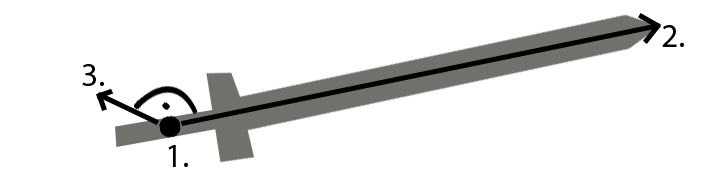
\includegraphics[width=140mm]{../img/diagram-swordPositioning.png}
  \caption{Diagram znázorňující kontrolní body meče}
  \label{obr05:swordPositioningDiagram}
\end{figure} 

Argument \textit{MoveSword()} má tedy tyto složky:
\begin{enumerate}
    \item \textbf{Poloha rukojeti} (Vektor) - poloha kam se má posunout anchor meče ve světových souřadnicích.
    \item \textbf{Směr meče} (Vektor) - přičtením k Poloze rukojeti dostaneme bod ve světových souřadnicích, kterým má čepel meče procházet.
    \item \textbf{Normála na čepel meče} (Vektor) - pro určení rotace meče kolem jeho osy. Kolmý na Směr meče. Obě hrany ostří čepele se budou nalézat v rovině určené Bodem rukojeti a touto normálou.   
    \item \textbf{Síla držení} (Číslo) - udává jak pevně má meč být držen ve své pozici.
\end{enumerate}

Polohu rukojeti jsme získali přímo, kvaternion pro rotaci vypočteme vestavěnou funkcí:

\begin{code}
 UnityEngine.Quaterion.LookRotation(
   forward: SmerMece,
   upwards: NormalaNaCepelMece
 )
\end{code}

Obě tyto hodnoty a rovněž Sílu držení poznamenáme v privátním stavu, odkud s nimi pracují mechanismy pro vykonávání pohybu.

\subsubsection*{Rotační pohyb} \label{implementationSwordAngularMovementSubsubsection}

Nejprve se podívejme odděleně na rotační složku pohybu. Tu bylo možné ponechat téměř zcela v režii ConfigurableJointu.

Na jointu bylo pouze třeba z editoru nakonfigurovat nenulový \textit{angularDrive} a všechny rotační stupně volnosti nastavit jako \textit{Free}. Následně již skript může přepisovat pole \textit{joint.targetRotation} a meč se sám silou jointu bude plynule pohybovat na danou pozici.

Této metodě nečiní problém ani fakt, že je cílová pozice každý snímek novým voláním \textit{MoveSword()} přepsána - každý snímek joint na meč aplikuje sílu posunující jej k té zrovna aktuální \textit{targetRotation}. 

Jediný větší problém, na který jsme zde narazili, je abnormální souřadnicový systém, který ConfigurableJoint pro targetRotation používá - převod z klasických světových souřadnic, které nám předala \textit{MoveSword()}, je složitější záležitost a věnujeme mu celou sekci \ref{howToSetJointsTargetRotationSection}. 

Rovněž bylo třeba vyladit parametry jak na rigidbody meče, tak nalézt vhodný \textit{angularDrive}. Následně jsem však získali meč, který je schopen velmi plynulého a celkově pěkného úhlového pohybu a nečiní mu problém ani být realisticky ovlivňován kolizemi s cizími předměty (např. být sražen pod úderem nepřátelského meče) - nad mírou této jeho schopnosti navíc máme vcelku značnou kontrolu skrze konfiguraci \textit{angularDrive} (čím větší \textit{spring}, tím více drží v cílové pozici).

\subsubsection*{Lineární pohyb}

Druhou složkou je lineární pohyb. Podívejme se nyní na ten.

Zde jsme se pokusili, analogicky jako u rotace, pro jednotlivé stupně volnosti nastavit joint jako \textit{Free} a polohu meče kontrolovat pomocí položky \textit{targetPosition}. Narozdíl od rotace, zde se však joint choval nestabilně - pokud jsme cílovou pozici odchýlili příliš daleko od kotvícího bodu, meč začal být v nepředvídatelných intervalech surově vystřelován do dáli. Příčinu takto rozbitého chování se nám nepodařilo odhalit, pro lineární pohyb meče jsme tedy raději zvolili alternativní metodu. 

Pomohla nám proměnná \textit{joint.connectedAnchor}. Ta udává pozici na těle šermíře, ke které je joint svým \textit{anchorem} ukotven. Defaultně je nastavená jako readonly - v editoru jí díky tomu joint může automaticky updatovat, aby souhlasila s nastavenou hodnotou \textit{anchor} a polohou ve světě, kam jsme meč umístili. Zapisovací práva získáme vypnutím\footnote{Vhodné je ho v editoru nechat zapnutý a vypnout jej až programaticky při inicializaci SwordMovement. Takto zachováme pohodlí při práci v editoru.} flagu \textit{joint.autoConfigureConnectedAnchor}. Nakonec je třeba nastavit všechny lineární stupně volnosti na \textit{Locked}.

Zápisem do \textit{joint.connectedAnchor} jsme nyní schopni meč okamžitě přesunout na cílovou pozici. My však potřebujeme pohyb plynule rozložený v průběhu času. 

Vyzkoušeli jsme několik řešení, která jsme následně zavrhli:
\begin{itemize}
  \item knihovnu DOTween - Ta neumožňuje změnit cílovou pozici jakmile tween začal
  \item externí objekt pohybovaný skrze fyzikální systém, na jehož pozici jsme hodnotu connectedAnchoru namapovali - Při dosažení cílové pozice objekt vykazoval jitter, který se nepodařilo odbourat.
\end{itemize}
Řešení, které jsme nakonec použili, bylo jednoduše každý FixedUpdate hodnotu connectedAnchoru posunout o malý zlomek její cesty k cíli - takto: 
\begin{code}
 joint.connectedAnchor += AnchorSpeed *
   (targetConnectedAnchor - joint.connectedAnchor) 
\end{code}
Parametr \textit{AnchorSpeed} je konfigurovaný z editoru. Vzhledem k tomu, že vše probíhá uvnitř FixedUpdate, pohyb je konzistentní.

Jde o velmi triviální řešení, jež neodpovídá realistickému fyzikálnímu chování, avšak pohyb meče se jeví plynule a hráčský zážitek se nezdá výrazněji trpět.

\subsubsection*{Síla držení meče} \label{implementationSwordHoldingForceSubsubsection}

Někdy je třeba kromě pozice meče mít kontrolu i nad způsobem, jak je meč držen. Např. v modu blokování potřebujeme, aby byl meč držen pevněji než při sekání, jinak by blokující meč byl tím sekajícím sražen na stranu (sekající se pohybuje a má tedy větší kinetickou sílu). 

Sílu držení meče jsme tedy umožnili definovat spolu s polohou. Jde o volitelný parametr - pokud není dodán, meč se navrací na defaultní sílu držení (která byla z jointu přečtena při inicializaci). Implementace probíhá jednoduše změnou položky \textit{joint.slerpDrive.spring}, používáme k tomu stejnou triviální interpolaci jako pro pohyb \textit{connectedAnchoru} výše.

\subsubsection*{Submoduly} \label{implementationSwordSubmodulesSubsubsection}

Již tedy máme představu, jak vnitřně probíhá pohyb meče. Nyní krátce k submodulům, které pro pohyb meče generují instrukce. 

Jak jsme nastínili v \ref{interfacesSwordMovementModulesObjectModelSubsubsection}, moduly jsou zvláštní typ entity, která nedědí z UnityEngine.Object, nýbrž je potomkem SwordMovement.Module. V editoru potřebujeme být schopni nakonfigurovat jeden defaultní modul a libovolně velkou množinu dalších, indexovanou jejich aktivačními klávesami.

Pro spravování indexované množiny objektů jsme implementovali třídu \textit{SerializableDictionary<TKey, TValue>} - ta obsahuje serializovatelný list key-value párů a umožňuje jeho jednoduchý převod na Dictionary. 

Vyvstává však problém - pole v tomto dictionary jsme deklarovali typu SwordMovement.Module - očekáváme, že konkrétní podtřídu vybere uživatel v editoru - Unity však v editoru výběr podtřídy nepodporuje. Naštěstí existuje knihovna SubclassPropertyDrawer \cite{SubclassPropertyDrawer}, která ji je schopna přímočaře doplnit.  

\begin{figure}[ht]\centering
  \center
  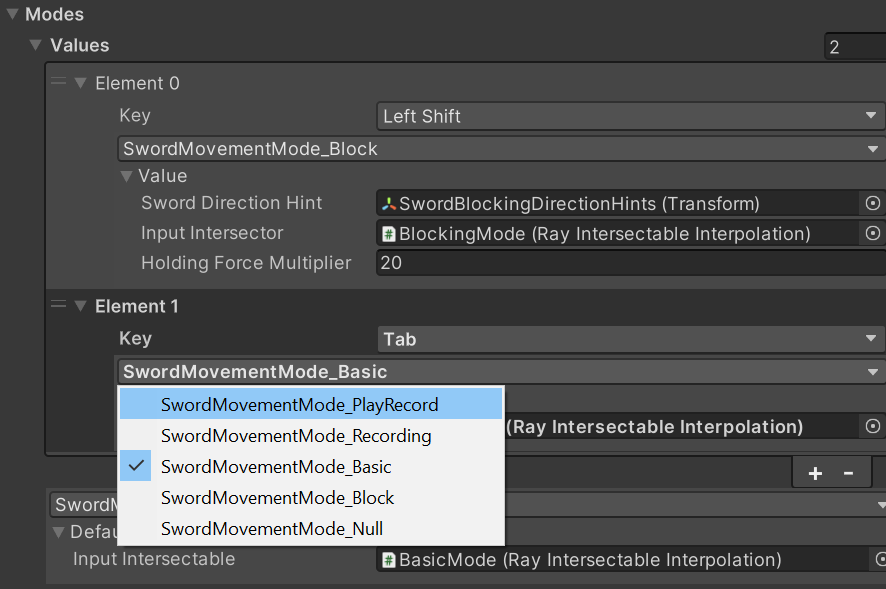
\includegraphics[width=110mm]{../img/swordMovementModulesEditor.png}
  \caption{Editace modulů v unity editoru}
  \label{obr05:swordModulePicker}
\end{figure} 

Správu životního cyklu modulů jsme oddělili do samostatné třídy \textit{ScriptSubmoduleListManager}. Té stačí dodat jejich indexovaný list a následně volat její updatovací callbacky jako by sama byla jediným aktivním modulem. O výběr a updatování aktivního modulu a vše s tím spojené se následně postará sama. 

Chceme-li tedy vytvořit dekorátor, který se vtěsná mezi SwordMovement a jeho moduly, stačí, aby dědil ze SwordMovement.Module a implementoval rozhraní \textit{ISwordMovement}. Původnímu SwordMovement nahradí jeho instanci \textit{ScriptSubmoduleListManager} za novou, ve které se nachází pouze on sám jako defaultní modul, a tu původní instanci ukradne pro sebe - jejím prostřednictvím může nyní originální moduly updatovat sám, aniž by se z jejich pohledu cokoliv změnilo.


\subsubsection*{Shrnutí}

Meč je šermířův nástroj interakce s okolím. Šermíř ho drží v jednom jeho daném bodě - kolem toho může meč rotovat, jeho přesunem se přesunuje meč v prostoru. Toto je umožněno použitím komponenty \textit{ConfigurabeJoint} - především rotační pohyb je díky ní plynulý a fyzikálně realistický. 

Instrukce k pohybu na konkrétní pozici získává meč od modulů své komponenty SwordMovement. Pro ty se nám podařilo umožnit, aby je mohl uživatel konfigurovat z editoru se značnou flexibilitou.

%------------------------------------------------------------------------------------------------------------------------------------------------------------------------------------------------------------------------------------------------------------%
 % xxxxxxxxxxxxxxxxxxxxxxxxxxxxxxxxxxxxxxxxxxxxxxxxxxxxxxxxxxxxxxxxxxxxxxxxxxxxxxxxxxxxxxxxxxxxxxxxxxxxxxxxxxxxxxxxxxxxxxxxxxxxxxxxxxxxxxxxxxxxxxxxxxxxxxxxxxxxxxxxxxxxxxxxxxxxxxxxxxxxxxxxxxxxxxxxxxxxxxxxxxxxxxxxxxxxxxxxxxxxxxxxxxxxxxxxxxxxxxxxxxxxxxxx %
%------------------------------------------------------------------------------------------------------------------------------------------------------------------------------------------------------------------------------------------------------------%


\subsection{Animace šermíře} \label{swordsmanAnimationSubsection}

Šermíře jsme si již navrhli jako kapsli, jež je schopna se působením fyzikálních sil pohybovat herním prostředím a ukotvit k sobě meč. Taková reprezentace je zcela v pořádku z programátorského hlediska, pro hráčův vizuální dojem však není ideální.

Proto jsme tedy v programu Blender \cite{Blender} vytvořili 3D model, který více připomíná humanoidního šermíře. V souladu se standardními postupy jsme mu vytvořili kostru a za její pomoci vytvořili velmi jednoduchou animaci dýchání. Následně jsme model importovali do Unity a umístili mezi potomky šermířského objektu.

Po správném napolohování tohoto detailního těla uvnitř šermířského objektu náš šermíř má adekvátní grafickou reprezentaci, která se pohybuje spolu s ním a je z ní patrné, na kterou stranu je šermíř obrácený. Nyní bychom mohli i přidat animace pro chůzi apod., mezi kterými by mohl přepínat \textit{SwordsmanMovement} v závislosti na aktuálně vykonávaném pohybu - manuální tvorba velkého množství animací však není cílem této práce, omezili jsme se tedy na cyklický běh animace dýchání. 

Detailní tělo dosud figuruje jako čistě kosmetický prvek, který se nijak neúčastní fyzikální simulace. Pokud bychom to takto ponechali, nepovede to k optimálnímu hernímu zážitku - hráč chce pravděpodobně protivníka zasahovat mečem do jeho těla, ne do jakési neviditelné obklopující kapsle. Na jednotlivé kosti\footnote{Rozmístěním colliderů na odpovídající kosti zaručíme, že se při animaci budou pohybovat korektně spolu s šermířovým modelem.} šermířova těla jsme tedy rozmístili komplexní systém colliderů - viz obr. \ref{obr05:swordsmanDetailedColliders}. Kolizní vrstvy jsme nakonfigurovali tak, aby tyto collidery kolidovaly pouze s meči ostatních šermířů, pro interakci s prostředím ponecháváme původní kapsli (té navíc samozřejmě vypneme kolize s meči). 

\begin{figure}[ht]\centering
  \center
  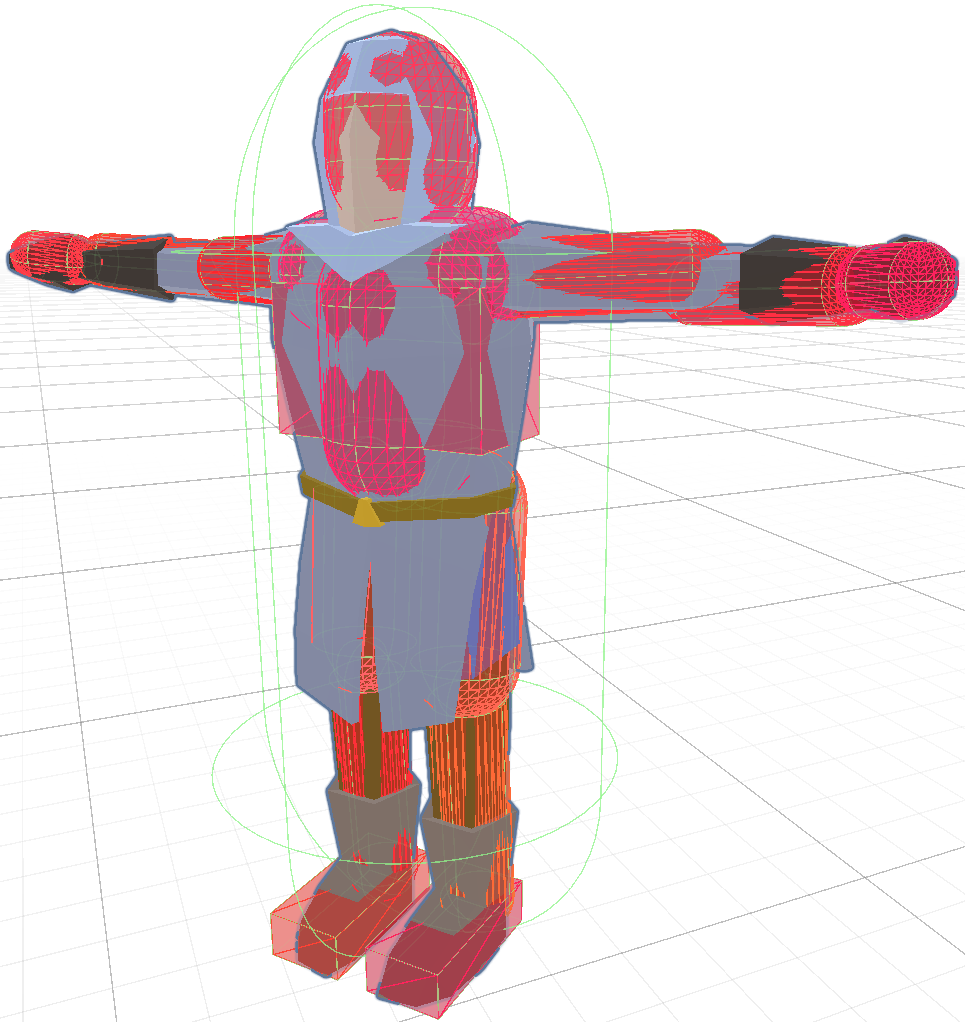
\includegraphics[width=90mm]{../img/swordsmanBodyColliders.png}
  \caption{3D model šermíře s collidery rozmístěnými na kostech}
  \label{obr05:swordsmanDetailedColliders}
\end{figure} 

Jednotlivými animacemi pro pohyb se zaobírat nebudeme, co však je zajímavým tématem, je zaručit, aby šermířovy ruce držely meč - ten se může pohybovat naprosto libovolně, není tedy možné použít předpřipravené animace. 

Zde nám pomůže knihovna Animation Rigging \cite{AnimationRigging}, která byla do Unity představena v nedávných letech. Ta nám poskytuje dodatečnou programovatelnou vrstvu nad vestavěným animačním systémem, skrze kterou můžeme animované objekty ovlivňovat. Najdeme zde mnoho již předpřipravených komponent, další lze vytvořit jako vlastní skripty.

Těžkou část práce za nás vykonala předpřipravená komponenta \textbf{TwoBoneIKConstraint}. Ta bere na vstupu bod značící cílovou pozici a pro řetězec tří navazujících kostí vypočítá pomocí algoritmu FABRIK \cite{FabrikSolverIK} polohování, které se tváří korektně z hlediska lidské anatomie, zachovává délku kostí a poslední z kostí se při něm nalézá v cílovém bodě. V našem případě oním cílovým bodem je bod, který jsme pro danou ruku vyznačili na rukojeti meče a řetězcem kostí je \textit{rameno -> loket -> dlaň}.

Pro každou šermířovu ruku jsme tedy vytvořili jednu tuto constraint. Na šermířovo tělo jsme následně umístili komponentu \textit{SwordsmanBodyProceduralAnimation}, jejímž úkolem je tyto constraints updatovat dle bodů získaných ze \textit{SwordDescriptoru}. 

Výsledek fungoval velmi dobře - šermířovy ruce skutečně meč na příslušných místech držely. Problém však nastal, pokud se meč ocitl příliš daleko mimo jejich dosah - v takovém případě nastávalo nedefinované chování. K vyřešení tohoto problému jsme tedy napsali dle instrukcí v dokumentaci vlastní constraint \textit{ExtendSwordsmanArmsToReachTheSwordConstraint}, která běží před TwoBoneIKConstraint a jednoduše kosti prodlouží, aby na cílovou pozici vždy dosáhly.


\begin{figure}[ht]\centering
  \center
  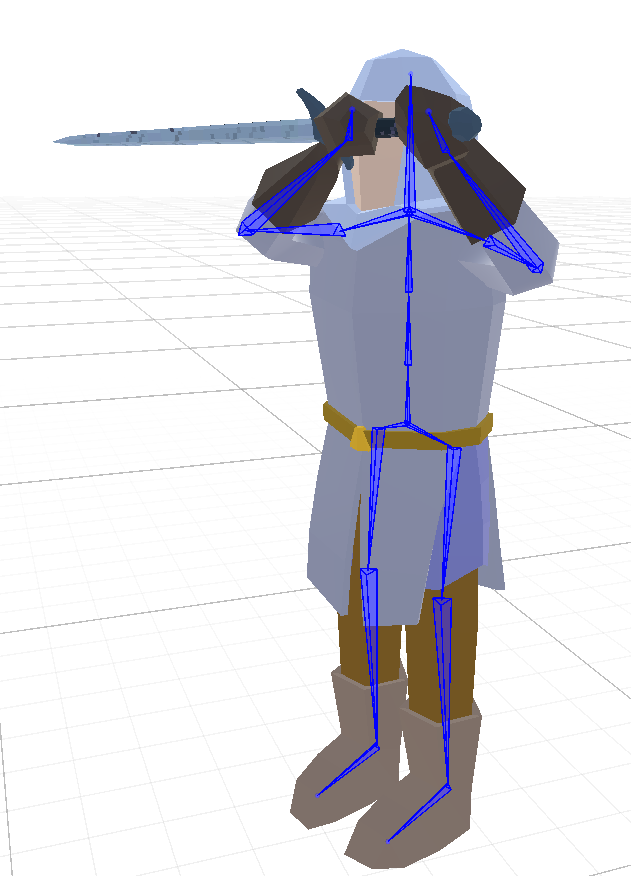
\includegraphics[width=80mm]{../img/swordsmanProceduralAnimation.png}
  \caption{Šermíř držící meč}
  \label{obr05:swordsmanProceduralAnimation}
\end{figure} 


\subsection{Systém zranění}

Systém zranění je protkán napříč celým naším návrhem, jeho fungování by již čtenáři mělo být zřejmé z předchozí kapitoly - stručně: 
\begin{itemize}
  \item \textbf{Damageable} definuje entitu, která může být zraňována a zemřít.
  \item \textbf{IArmorPiece} sídlí v podobjektu Damageable, spravuje konkrétní množinu colliderů a zpracovává útok učiněný na tyto collidery .
  \item \textbf{Zbraň} je cokoliv, co umí najít odkaz na IArmorPiece a zavolat na něm metodu ProcessAttack().
\end{itemize}
Zde velmi stručně projdeme implementaci jednoduché zbraně a zbroje, které náš systém používá.

\subsubsection*{BasicArmorPiece}

Odkaz na své Damageable najde prohledáváním hierarchie směrem nahoru. Definuje dva parametry:
\begin{itemize}
  \item \textit{Násobič zranění} - číslo kterým vynásobí dmg útoku  
  \item \textit{Minimální zranění} - pokud je výsledné dmg pod touto hranicí, útok bude ignorován
\end{itemize}

Jeho metoda ProcessAttack() spočte výsledné dmg a pokud je nad minimální hranicí, ubere toto množství HP svému Damageable voláním ChangeHP().

Šermířovi jsme umístili jednu instanci do kořenu jeho detailního těla - ta definuje základní chování pro všechny jeho collidery - do kostí jeho rukou jsme umístili dvě doplňující instance s menším násobičem. Ruce budou veškeré zásahy defaultně zpracovávat těmito v hierarchii bližšími instancemi, čímž se kompenzuje jejich jinak nadprůměrná zranitelnost. Podobně by se dal vyladit i zbytek šermířova těla.

\subsubsection*{BasicImpactWeapon}

Jednoduchá na fyzice založená zbraň. Definuje tyto parametry:
\begin{itemize}
  \item \textit{Násobič zranění} - číslo kterým vynásobí dmg útoku 
  \item \textit{Čas mezi útoky} - minimální interval mezi dvěma útoky na stejnou entitu
\end{itemize}

Poslouchá na zprávy OnCollisionEnter. Při každé kolizi se pokusí na zasaženém collideru najít komponentu IArmorPiece prohledáváním hierarchie nahoru - pokud nějakou najde a její Damageable není v jeho interním seznamu\footnote{Pro každé Damageable si interně vede timestamp posledního zásahu. Na pozadí běží korutina, která pravidelně záznamy s prošlou platností maže, aby nedocházelo k memory leakům.} entit zasažených v posledních \textit{ČasMeziÚtoky} sekundách, vykoná útok voláním ProcessAttack(). Dmg je vypočteno z argumentu kolizního callbacku jednoduše jako síla kolize (\textit{collision.impact.magnitude}) násobená s \textit{Násobičem} nastaveným z editoru, jako bod útoku je hlášen 1. bod kolize (\textit{collision.GetContact(0)}). 

Vzhledem k tomu, že je komponentou poslouchající na OnCollision zprávy, musí se nacházet v kořenovém objektu zbraně spolu s Rigidbody (viz \ref{collidersPhysicsIntroSubsection}) a není možné ji omezit pouze na specifickou množinu colliderů. Meč tedy nutně způsobuje stejné zranění při zásahu čepelí i při zásahu záštitou či rukojetí. Rovněž tato implementace nerozlišuje, zda byl zásah vykonán plochou či ostrou stranou čepele - chová se efektivně jako kyj či podobná tupá zbraň. 

Pro účely této práce se však současný systém jeví jako dostačující. Implementaci realističtějšího výpočtu zranění, který umožní rozlišení mezi ostrou a plochou stranou čepele, záštitou a rukojetí, ponecháme pro navazující práce. 

\pagebreak
%------------------------------------------------------------------------------------------------------------------------------------------------------------------------------------------------------------------------------------------------------------%
 % xxxxxxxxxxxxxxxxxxxxxxxxxxxxxxxxxxxxxxxxxxxxxxxxxxxxxxxxxxxxxxxxxxxxxxxxxxxxxxxxxxxxxxxxxxxxxxxxxxxxxxxxxxxxxxxxxxxxxxxxxxxxxxxxxxxxxxxxxxxxxxxxxxxxxxxxxxxxxxxxxxxxxxxxxxxxxxxxxxxxxxxxxxxxxxxxxxxxxxxxxxxxxxxxxxxxxxxxxxxxxxxxxxxxxxxxxxxxxxxxxxxxxxxx %
%------------------------------------------------------------------------------------------------------------------------------------------------------------------------------------------------------------------------------------------------------------%


\section{Stabilita simulace} \label{simulationStabilitySection}

Nyní by čtenář měl mít hrubý přehled o celkovém vnitřním fungování našeho systému. V této sekci se do detailu zaměříme na nečekané překážky, které nám v průběhu implementace postavil do cesty fyzikální subsystém, a vysvětlíme, jakým způsobem byly překonány.

\subsection{Jak nastavit cílovou rotaci jointu} \label{howToSetJointsTargetRotationSection}

V \ref{implementationSwordAngularMovementSubsubsection} jsme zmínili, že ConfigurableJoint používá pro svůj parametr \textit{targetRotation} velmi nestandardní souřadnicový systém. Jeho analýzu za nás naštěstí již vykonal \cite{ConfigurableJointExtensions} uživatel portálu github jménem mstevenson. Protože však jeho algoritmus pro nastavení rotace udávané v klasických světových či lokálních souřadnicích existuje pouze ve formě webové stránky, zde ho pro archivní účely také ukážeme: 

\begin{code}
void SetTargetRotation(
 ConfigurableJoint joint, //joint na kterém nastavujeme rotaci 
 Quaternion targetRotation, //rotace kterou chceme nastavit
 Quaternion startRotation, //rotace se kterou byl joint vytvořen
 Space space //lokální nebo globální souřadnice
)
{
 // Nejprve vypočteme báze interního souřadnicového systému
 var right = joint.axis;
 var forward = joint.axis.CrossProduct(joint.secondaryAxis).normalized;
 var up = forward.CrossProduct(right).normalized;
 var ordinaryToJointSpace = Quaternion.LookRotation(forward, up);
 
 //Rotace se v jointových souřadnicích chová inverzně
 targetRotation = targetRotation.inverse;

 //Transformace ze souřadnic jointu do klasických
 var resultRotation = ordinaryToJointSpace.inverse;

 //Aplikujeme počáteční rotaci a cílovou rotaci
 switch(space){
  case Space.World:
    resultRotation *= startRotation * targetRotation;
    break;
  case Space.Local:
    resultRotation *= targetRotation * startRotation;
    break;
 }
 //Návrat zpět do souřadnic jointu
 resultRotation *= ordinaryToJointSpace;
 
 //Nastavíme rotaci
 joint.targetRotation = resultRotation;
 }
\end{code}

Zda smíme používat světové, nebo lokální souřadnice, záleží na hodnotě flagu \textit{joint.configuredInWorldSpace}. Argument \textit{startRotation} je (buď globální, nebo lokální) rotace, kterou jsme přečetli z \textit{joint.transform} na začátku hry ve zprávě Start().

V případě našeho meče používáme lokální souřadnice. Tedy \textit{joint.configuredInWorldSpace} musí být false a jako parametr \textit{startRotation} posíláme \textit{joint.transform.localRotation}.

V naší práci jsme tuto logiku zapouzdřili do třídy \textit{JointRotationHelper}, kterou je třeba inicializovat odkazem na joint při spuštění hry. Následně pro nastavení cílové rotace stačí volat její metodu \textit{SetTargetRotation} s jediným argumentem udávajícím cílovou rotaci.


\subsection{Ladění parametrů} \label{swordParameterTweaksSection}

Fyzikální objekty poskytují mnoho parametrů, které ovlivňují jejich chování. K dosažení dobrého výsledku bylo nutné strávit dlouhý čas jejich laděním. Pro mnoho z těchto parametrů je jejich přesný význam v oficielní dokumentaci nastíněn jen mlhavě, např. použitá jednotka často není vůbec udána. V kombinací s inherentní nepřesností fyzikální simulace tedy nebylo možné pouze přepsat do hry obraz reality - k nalezení vhodných parametrů často neexistovala lepší cesta než binární vyhledávání či podobné heuristiky. Vzhledem k tomu, že funkcí posuzující kvalitu chování byl pouze subjektivní dojem, a že rovněž parametry často ovlivňují jeden druhý, zcela jistě jsme nenašli jejich optimální ohodnocení. Přesto jsme se však dobrali k výsledku, který se zdá plynout v přijetelný herní zážitek. Ten si nyní představíme.

\bigbreak
Nejprve bylo třeba meči a šermířovi stanovit váhu. Její jednotka je v oficielní dokumentaci udána jako kg, mohli jsme ji tedy nastavit zhruba realisticky - pro šermíře \textit{60}, pro meč \textit{1.5}.

\subsubsection*{Svižnost sekání}

Pro dosažení svižného pohybu meče bylo třeba poladit parametry jak na \textit{Rigidbody} meče, tak na jeho \textit{ConfigurableJointu}:
\begin{itemize}
  \item \textit{joint.rotationDriveMode = Slerp} - takto se meč do cílové pozici přesunuje vždy nejkratší cestou
  \item \textit{joint.slerpDrive = {spring: 120, damper: 10}} - hodnoty pro mod sekání. Spring musí být cca o jeden až několik řádů větší než damper, aby se meč pohyboval svižně a pevně držel pozici, příliš malý damper způsobí ošklivý třas.
  \item \textit{rigidbody.centerOfMass = joint.anchor} - těžiště by mělo být poblíž bodu ve kterém šermíř meč drží.
  \item \textit{rigidbody.inertiaTensor = (0.05, 0.05, 0.02)} - velmi malé ale nenulové\footnote{Dle \href{https://docs.unity3d.com/ScriptReference/Rigidbody-inertiaTensor.html}{oficielní dokumentace} 0 je zde ekvivalentní nekonečnu.} hodnoty. Určuje lehkost, s jakou meč rotuje v jednotlivých osách.
  \item \textit{rigibody.centerOfMass, rigidbody.inertiaTensor} - nutně musí být nastavené manuálně z editoru. Jinak je balanc zcela rozbit\footnote{Defaultně fyzikální systém tyto dvě hodnoty automaticky přepočítává podle rozmístění colliderů. Collidery přidané korekcí kolizí jsou velmi neforemné.} při použití korekce kolizí (viz \ref{swordCollisionsSection}).
  \item \textit{joint.massScale = 9} - zvýšilo subjektivní svižnost a pádnost meče.
  \item \textit{rigidbody.useGravity = false} - konzistentnější chování meče napříč směry pohybu.
\end{itemize}

\subsubsection*{Přenos sil mezi mečem a šermířem}

Dále bylo nutné zařídit, aby síly, které na meč působily, nebyly příliš moc přenášeny na šermíře. Samotná síla, kterou vynakládal joint ke švihání meče, jinak stačila na to, aby byl šermíř citelnou rychlostí neustále ''tahán'' dopředu.

Problém jsme vyřešili nastavením malé \textit{joint.connectedMassScale} - konkrétně jsme použili hodnotu \textit{0.01}.

\subsubsection*{Stabilita simulace}

Případy obecně podivného chování jsme zredukovali nastavením těchto parametrů:
\begin{itemize}
  \item \textit{joint.enablePreprocessing = false} - celkově zlepšilo stabilitu.
  \item \textit{joint.projectionMode = PositionAndRotation} - když je poloha, kde se meč má vyskytovat, nesplnitelná, takto se místo nevyzpytatelného chování přesune na místo poblíž šermíře - fyzikálně nerealisticky, leč úhledně.
\end{itemize}


\subsubsection*{Síla držení meče}

Při použití stejného \textit{joint.slerpDrive} pro mod sekání i mod blokování byl blok blokujícího meče tím sekajícím konzistentě prorážen. Bylo tedy třeba nějak zvýšit ''sílu, kterou je blokující meč držen''. 

Po testování jsme došli k závěru, že pro blokovací mod fungují adekvátně tyto parametry:
\begin{itemize}
  \item \textit{joint.slerpDrive.spring: 2400}
  \item \textit{joint.slerpDrive.damper: 5}
\end{itemize}

Při přepínání mezi mody ovládání pro tyto parametry vykonáváme plynulý přechod - viz \ref{implementationSwordHoldingForceSubsubsection}. Blokování je takto proti sekajícímu meči účinné, jinak si meč stále zachovává své klasické chování.


\pagebreak
%------------------------------------------------------------------------------------------------------------------------------------------------------------------------------------------------------------------------------------------------------------%
 % xxxxxxxxxxxxxxxxxxxxxxxxxxxxxxxxxxxxxxxxxxxxxxxxxxxxxxxxxxxxxxxxxxxxxxxxxxxxxxxxxxxxxxxxxxxxxxxxxxxxxxxxxxxxxxxxxxxxxxxxxxxxxxxxxxxxxxxxxxxxxxxxxxxxxxxxxxxxxxxxxxxxxxxxxxxxxxxxxxxxxxxxxxxxxxxxxxxxxxxxxxxxxxxxxxxxxxxxxxxxxxxxxxxxxxxxxxxxxxxxxxxxxxxx %
%------------------------------------------------------------------------------------------------------------------------------------------------------------------------------------------------------------------------------------------------------------%


\subsection{Kolize mečů} \label{swordCollisionsSection}

Jednou z největších výzev, které bylo v průběhu práce třeba překonat, je zajištění korektního chování kolizí při srážce dvou mečů.


\subsubsection*{Problematika detekce kolizí}

V \ref{collidersPhysicsIntroSubsection} jsme již velmi letmo nastínili typicky používanou metodu diskrétní detekce kolizí a problém tunelování, který je jejím důsledkem. Pro zopakování - jde o jev, kdy malý či rychle se pohybující objekt projde skrze překážku, která mu stojí v cestě, aniž by byla detekována jejich kolize.

Typickým herním žánrem, kde na tento problém narážíme velmi často, jsou \acs{FPS} hry. Vystřelené projektily jsou obvykle malé a zároveň se pohybují velmi rychle - v kompetitivní střílečce by bylo velmi nežádoucí, kdyby nepředvídatelně některé střely byly schopné trefovat hráče skrz zeď, či naopak jimi projít aniž by je zranily.  

Pro řešení tohoto specifického problému moderní fyzikální systémy typicky nabízejí alternativní metody detekce kolizí - tzv. spojité - které lze zapnout pro konkrétní herní objekty, které je potřebují. Vestavěný fyzikální systém v Unity v tomto ohledu není výjimkou.


\subsubsection*{Náš problém}

Podobně jako projektily ve střílečce, naše meče jsou rovněž relativně malými objekty, které se pohybují vcelku rychle. Používáme-li diskrétní detekci kolizí, není překvapením, že při srážce dvou mečů často k tunelování dojde. Tím přirozeně velmi trpí možnost blokovat nepřátelské údery a celkově nejde o dobrý stav, který by napomáhal hráčské imerzi.

\bigbreak

Zkusili jsme tedy pro meče aktivovat spojitou detekci kolizí - pro tu Unity nabízí dvě různé metody. První, kterou jsme zkusili, je \textbf{spojitá dynamická}.

Ta však náš problém nevyřešila. Výskytů tunelování citelně ubylo, stále se však příležitostně objevily. I v případě, že kolize byla zdetekována, se však meč nechoval dle očekávání - místo aby se od sebe meče odrazily, nastal efekt jakéhosi jejich zamrznutí na místě. Zkrátka síly aplikované na oba meče k rozřešení kolize nebyly korektní.

Důvod tohoto chování najdeme v oficielní dokumentaci. Tam se dočteme, že spojitá dynamická detekce kolizí bere v úvahu pouze lineární pohyb objektů, rotační složku zcela ignoruje. To nečiní problém v typické situaci letícího projektilu, v případě našich mečů je to však silně nežádoucí.  

\bigbreak

Záchranou by mohla být druhá metoda - \textbf{spojitá spekulativní} detekce kolizí. Ta dle dokumentace bere v úvahu lineární i úhlový pohyb, měla by také být rychlejší a jediné negativum je, že příležitostně mohou být detekovány dodatečné neexistující kolize. 

Překvapivě však po její aktivaci tunelování nastávalo téměř stejně často jako při diskrétní detekci. Krokováním hry po snímcích s fyzikálním debuggerem jsme odhalili, že kolize jsou skutečně detekovány, síla použitá na jejich rozřešení však meče pošle přesně opačným směrem než by měla - místo aby jejich protunelování zabránila, naopak mu pomůže. Toto stejné chování jsme zpětně odhalili i v mnoha případech tunelování při diskrétní detekci kolizí.


\subsubsection*{Možnosti řešení}

Metody detekce kolizí, které Unity poskytuje, jsou tedy očividně stavěné pro velmi specifické způsoby použití, v atypické situaci našich mečů mnoho nepomohou. Musíme tedy najít vlastní cestu, jak korektní chování při kolizích zaručit. 

Pro jednoduchost zatím předpokládejme, že ve hře figurují právě dva meče. Po krátkém zamyšlení jsme navrhli tato řešení:
\begin{itemize}
  \item \textbf{Každý snímek ručně testovat, zda meče prošly skrz, a manuálně je vracet}\linebreak
    Detekovat, zda meče prošly skrz, není těžký problém\footnote{Meče zjednodušíme na dvě úsečky v prostoru.}. Velmi obtížně uchopitelný úkol však je určit správně síly, které by ke korektnímu rozřešení této kolize bylo třeba aplikovat.
  \item \textbf{Poslouchat na kolize a manuálně meče vracet}\linebreak
    Jak jsme si nastínili výše, spojitá spekulativní metoda kolize většinou detektuje, pouze je rozřeší opačně než by měla. Mohli bychom tedy poslouchat na kolizi a v případě, že má být rozřešena špatně, zkrátka na meče aplikovat opačnou sílu a tím tunelování zvrátit.
  \item \textbf{Přidat velký neviditelný collider, který meči zabrání projít skrz}\linebreak 
    Takto bychom úkol detekce kolize i aplikování správné síly pro její rozřešení přenesli zpět na fyzikální systém. Bylo by však třeba tento collider polohovat, aby meči stál v cestě správným způsobem, a zařídit, aby nekolidoval s ničím dalším.  
\end{itemize}

Letmo jsme vyzkoušeli druhou metodu, ukázalo se však, že síly, které jsou v OnCollision callbacku pro kolizi hlášeny, se silám, kterými byla kolize reálně rozřešena, blíží jen velmi vzdáleně. Nebyli jsme tedy schopni dosáhnout jakkoliv stabilního a realisticky se tvářícího chování. Navíc příležitostně stále docházelo k tunelování, které žádnou kolizi nedetekovalo.

\bigbreak

Po krátké úvaze jsme se rozhodli pokračovat metodou dodatečného collideru.

%>---------------------------------------------------------------------------------------------------------------------------------------------------------------------------------------------------------------------------------------------------------------------------------<%


\subsubsection*{Implementace - geometrický popis}

Nejprve zavedeme definice, se kterými budeme pracovat:
\begin{itemize}
  \item \textbf{Meč} - úsečka v 3D prostoru odpovídající středové ose meče, začíná ve špičce čepele a končí v rukojeti
  \item \textbf{Fixovací collider} (zkráceně fixer) - collider který umísťujeme 
  \item \textbf{Hostitel} - meč, do kterého fixer umísťujeme
  \item \textbf{Cíl} - meč, kterému se fixer snaží zabránit, aby skrz hostitele protuneloval
\end{itemize}

Náším cílem je fixer umísťovat tak, aby došlo k jeho kolizi s Cílem tehdy a právě tehdy, když Cíl koliduje i s Hostitelem. Tedy celé jeho tělo by se mělo od hostitele nacházet vždy na opačné straně, než se nachází Cíl, a Hostitel by měl procházet jeho okrajem - viz obr. \ref{obr05:fixerBirdseye}. 
\begin{figure}[ht]\centering
  \center
  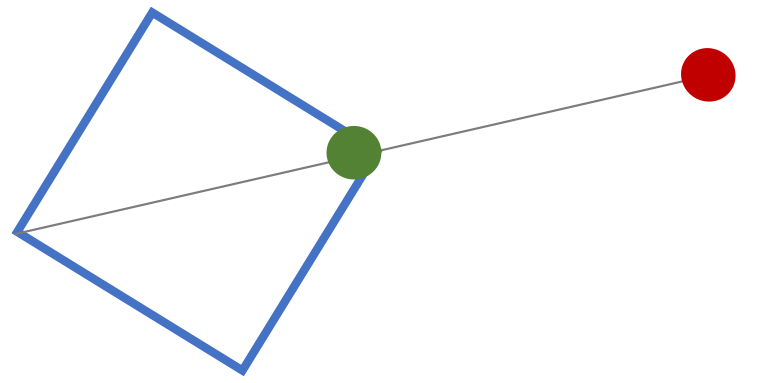
\includegraphics[height=30mm]{../img/fixerBirdseye.png}
  \caption{Z ptačí perspektivy - Hostitel (zeleně), Cíl (červeně), Fixer (modře)}
  \label{obr05:fixerBirdseye}
\end{figure} 
Z tvarů, které nám nabízejí primitivní collidery, se pro tento účel jeví nejvhodnějším BoxCollider. Jeho výšku stanovíme shodnou s délkou meče - jedna z jeho vertikálních hran se bude s osou Hostitelského meče shodovat - podstavu necháme pro jednoduchost čtvercovou a délku hrany necháme uživatelsky parametrizovatelnou - my budeme dále pracovat s pojmem \textbf{Hloubka}... vzdálenost jednoho z vrcholů podstavy od jejího středu - tedy polovina úhlopříčky podstavy.
\begin{figure}[ht]\centering
  \center
  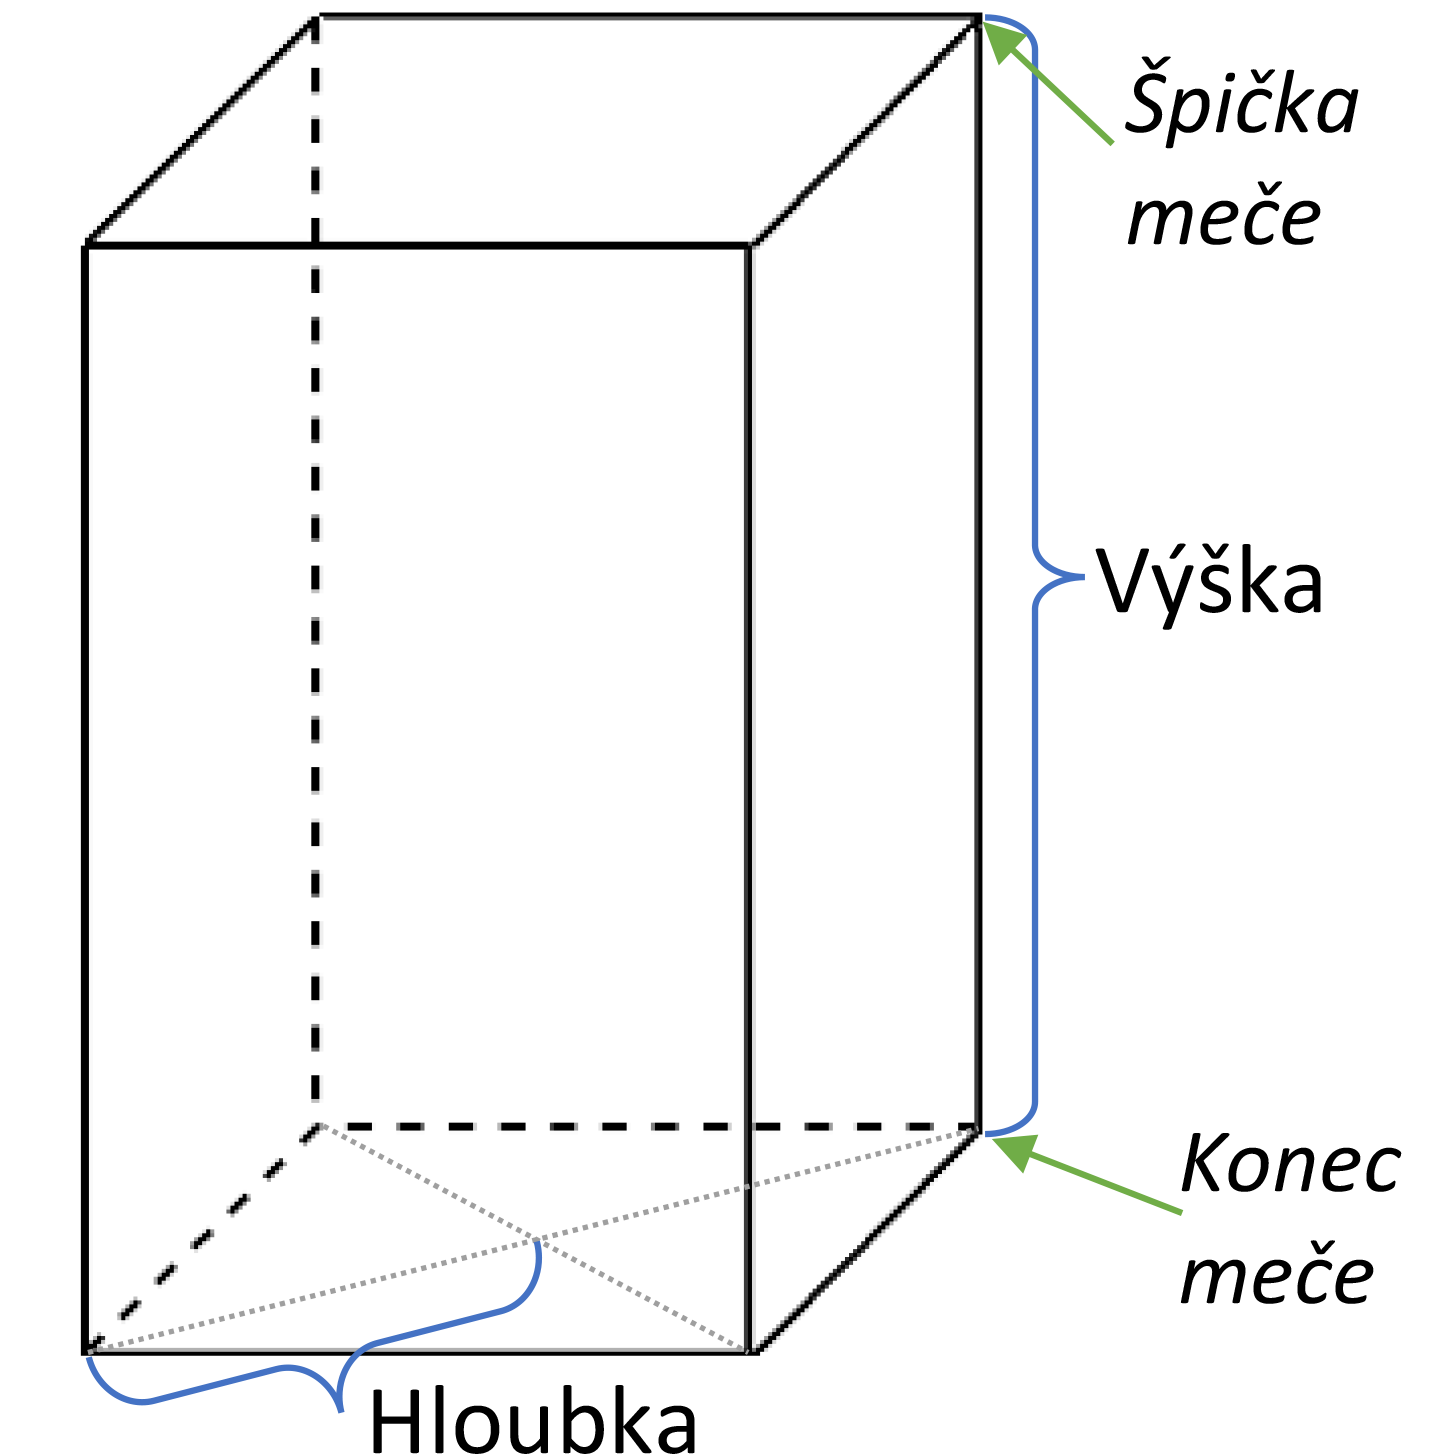
\includegraphics[height=70mm]{../img/fixerDefinitions.png}
  \caption{Rozměry fixeru}
  \label{obr05:fixerDefinitions}
\end{figure} 

Myšlenku tedy máme, jak však pro dvě obecné úsečky v prostoru definujeme ''na opačné straně''?

\bigbreak

Máme-li přímku a bod, úkol je jednoduchý. Provedeme zkrátka projekci bodu na přímku. Odečtením bodu od jeho projekce získáme \textbf{směr}, který z přímky ukazuje přesně na opačnou stranu. Bod, kam je třeba umístit střed fixeru, následně získáme vynásobením tototo směru s Hloubkou a přičtením ke středu Hostitelského meče. Výpočet rotace je srovnatelně jednoduchý - celkově:   

\begin{code}
fixer.position = 
  (hostitel.begin + hostitel.end)/2 
  + směr.normalized * fixer.hloubka;
fixer.rotation = 
  Quaternion.AngleAxis(45, hostitel.direction)
  * Quaternion.LookRotation(forward: směr, up: hostitel.direction);
\end{code}
Při pohledu na meč z ptačí perspektivy by výsledek odpovídal obr. \ref{obr05:fixerBirdseye}. 

\bigbreak

Naším protějškem je však úsečka. Bylo by možné převést naši situaci na předchozí případ nalezením nějakého vhodného reprezentativního bodu?

Nejprve jsme zkusili vybrat na Cílovém meči nějaký pevný bod - např. střed nebo jeden z jeho krajů. To však nefungovalo - našli jsme mnoho případů, kdy se fixer natočil tak, že zkolidovala část jeho těla s částí Cílového meče, která se Hostitele vůbec nedotýkala. Čím vzdálenější byl reprezentativní bod od bodu čepele, kterým se Cílový meč dotýkal Hostitele, tím bylo natočení fixeru horší.

Poslední zmíněné pozorování nás navedlo na myšlenku, která se nakonec ukázala být ideálním řešením - nalézt \textbf{nejkratší spojnici} obou mečů. Bod Cílového meče, který na ní leží, by mohl být naším vhodným reprezentantem. Pokud spolu meče kolidují, zcela jistě to je v tomto bodě. Zkusme proti němu tedy fixer namířit. 

\bigbreak

Nejkratší spojnici mečů nalezneme následujícím způsobem:

Nejprve vypočteme její směr. Protože to je jejich nejkratší spojnice, musí být na přímky obou mečů kolmá:
\begin{code}
 Spojnice.direction = Hostitel.direction.CrossProduct(Cíl.direction);
\end{code}

Nejkratší spojnice prochází oběma přímkami. Víme tedy, že pro nějaké parametry \textit{t1}, \textit{t2} leží oba body
\begin{code}
 h := Hostitel.origin + t1 * Hostitel.direction,
 c := Cíl.origin + t2 * Cíl.direction
\end{code}
na naší spojnici. Jeden z těchto bodů si můžeme vybrat a označit ho za počátek naší přímky. Po zavedení parametru \textit{t3} pak s jeho pomocí můžeme vyjádřit druhý z bodů - takto:
\begin{code}
  c = h + t3 * Spojnice.direction
\end{code}
A takto rovnici můžeme rozepsat
\begin{code}
 Cíl.origin + t2 * Cíl.direction =
 (Hostitel.origin + t1 * Hostitel.direction) + t3 * Spojnice.direction
\end{code}
Všechny parametry \textit{.origin} a \textit{.direction} jsou nám známé 3D vektory, rozepsáním pro jednotlivé složky \textit{x}, \textit{y}, \textit{z}, tedy získáváme soustavu tří lineárních rovnic o 3 neznámých \textit{t1}, \textit{t2}, \textit{t3}. Tu řešíme klasicky použitím Gaussovy eliminace. Její vyladěnou a numericky stabilní implementaci nám poskytla knihovna Math.NET Numerics \cite{MathDotNetNumerics}.

Nyní známe hodnotu \textit{t2}. Tu osekáme do intervalu [0;1]\footnote{Předpokládáme, že pole \textit{.direction} jsou definována jako (\textit{end - origin}), bez normalizace.}, abychom místo nejkratší spojnice přímek získali nejkratší spojnici úseček, kterými meče jsou, a následně dosazením do rovnice pro bod \textit{c} získáme bod, který poslouží jako reprezentant Cílového meče. Výsledné chování fixeru lze vidět na obr. \ref{obr05:fixerPositioning}.


\begin{figure}[ht]\centering
  \center
  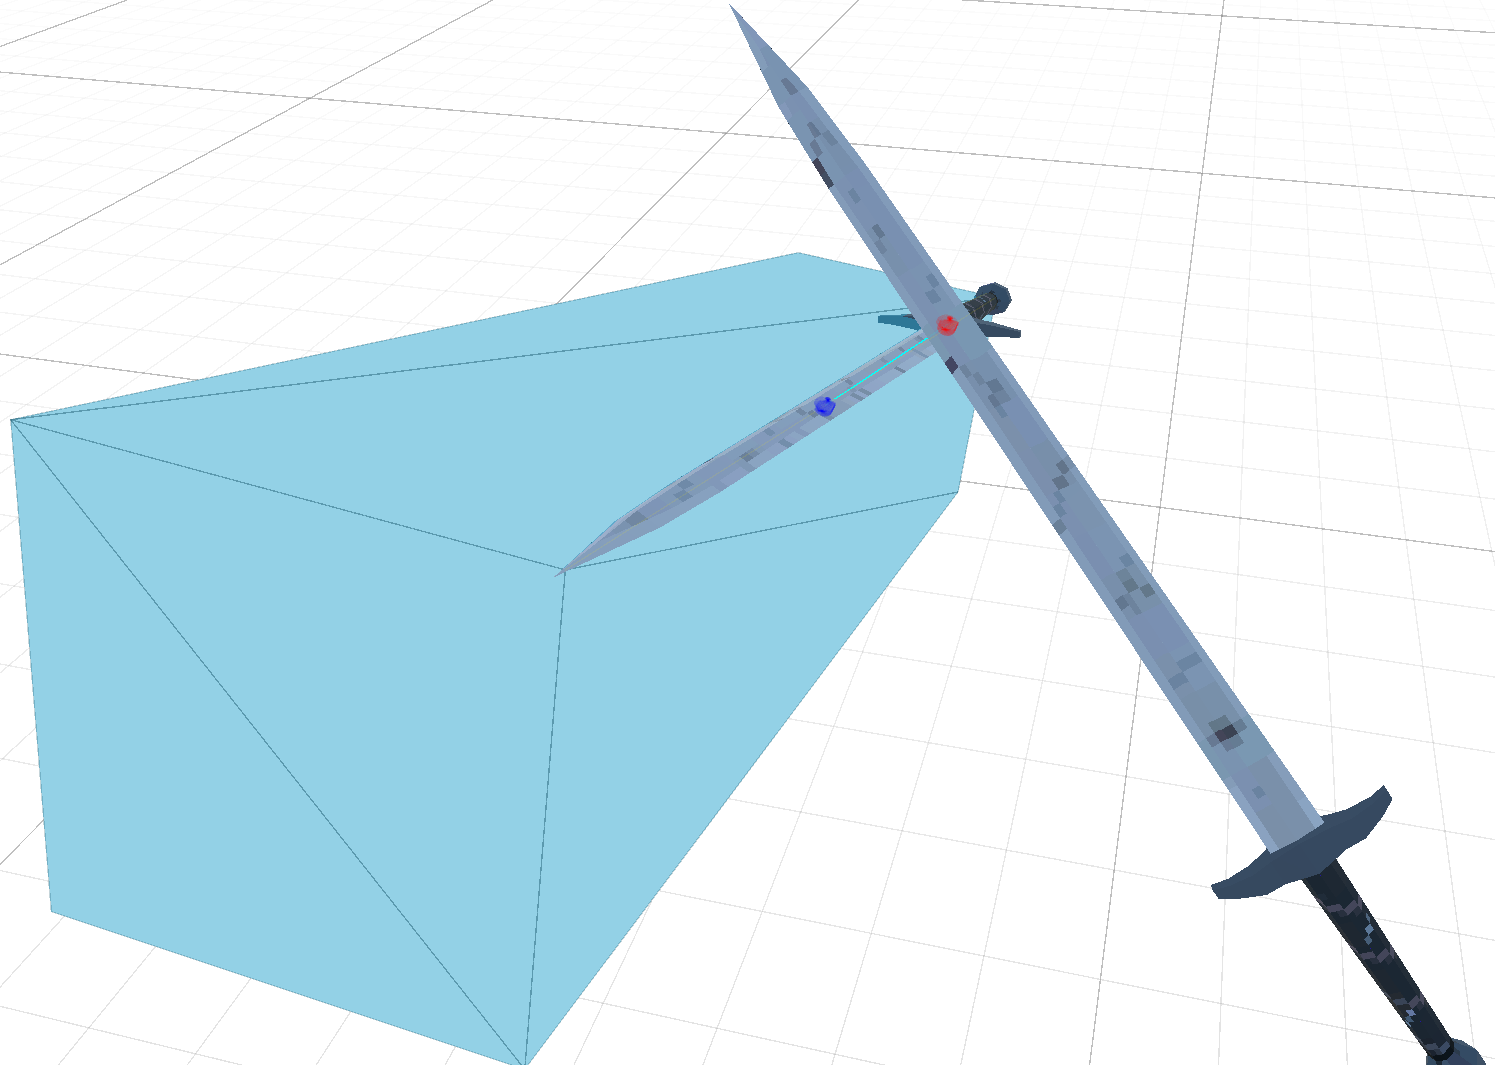
\includegraphics[height=90mm]{../img/collisionFix-show1.png}
  \caption{Výsledné polohování fixeru (barevně konce nejkratší spojnice)}
  \label{obr05:fixerPositioning}
\end{figure} 

Implementovali jsme herní komponentu \textit{ContrarianCollider}, která pro stanovený pár mečů vytvoří fixer a každý FixedUpdate nastavuje jeho pozici způsobem, který jsme si ukázali.


\subsubsection*{Implementace - neočekávané problémy}

Při testování jsme narazili na několik problémů. Prvním bylo, že fixer proti tunelování nijak nechránil. Jakmile Cílový meč protuneloval na opačnou stranu Hosta, fixer se rovněž okamžitě přetočil na opačnou stranu - dle předpisu, aby Cíli byl naproti - čímž mu přestal stát v cestě. Řešení naštěstí bylo jednoduché - v polohovacím skriptu jsme si zapamatovali spojnici mečů z předchozího snímku. Pokud se mezi snímky ostře změnila - skalární součin současného a minulého směru byl záporný - tak jsme směr té současné obrátili a dále pracovali s tím.
\begin{code}
  if(minuláSpojnice.direction.DotProduct(spojnice.direction))
    spojnice = nová Úsečka(spojnice.origin, -spojnice.direction);
  minuláSpojnice = spojnice;
\end{code}
Následně již fixer Cílovému meči v tunelování korektně bránil. Příležitostně však nastávaly situace, kdy tato podmínka byla vyhodnocena jako \textit{true}, aniž by šlo o tunelování. Např. okamžitě po inicializaci, v prvních několika snímcích hry, se celá hra zdá chovat celkově nestabilně a k tomuto jevu docházelo. Poloha fixeru se v takovém případě přepnula do stavu, kdy nastavoval směrem k Cílovému meči celý masiv svého těla - viz obr. \ref{obr05:fixerOverturned} - a docházelo tedy k pro hráče velmi matoucím kolizím s neznámým neviditelným objektem. 

\begin{figure}[ht]\centering
  \center
  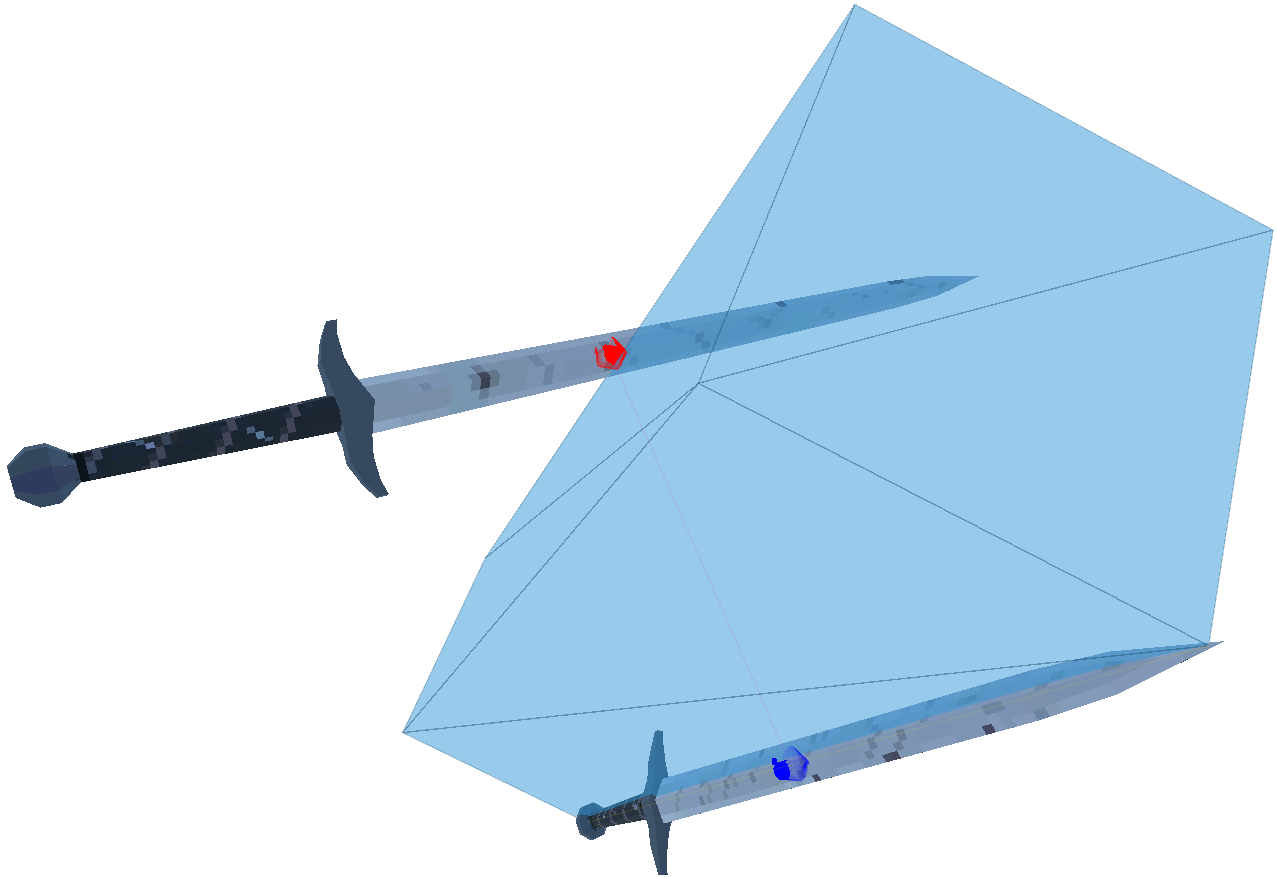
\includegraphics[height=90mm]{../img/fixerOverturned.png}
  \caption{Fixer s převráceným směrem}
  \label{obr05:fixerOverturned}
\end{figure} 

Přidali jsme tedy číselný parametr: \textit{Maximální vzdálenost detekce tunelování} - pokud byla délka spojnice obou mečů větší než tento parametr, převracení jejího směru jsme nevykonávali. Pokud by i tak k převrácení směru fixeru někdy došlo, stačí nyní od Cílového meče odstoupit na tuto vzdálenost a vše se srovná do standardního stavu. 

\bigbreak

Dalším problémem, na který jsme narazili, bylo, že příležitostně Cílový meč protuneloval na druhou stranu Hosta a ''skřípl'' se mezi něj a fixer - viz obr. \ref{obr05:fixerSqueak}. Řešením bylo fixeru přidat \textit{přesah} - dodatečnou velikost, kterou collider fyzicky má, avšak není brána v úvahu při geometrických výpočtech. Hrana fixeru takto tedy neprochází přesně středovou osou meče, ale přesahuje dál - viz obr. \ref{obr05:fixerOverreach} - čímž se prostor pro skřípnutí druhého meče drasticky zmenšuje. 

\begin{figure}[ht]\centering
  \center
  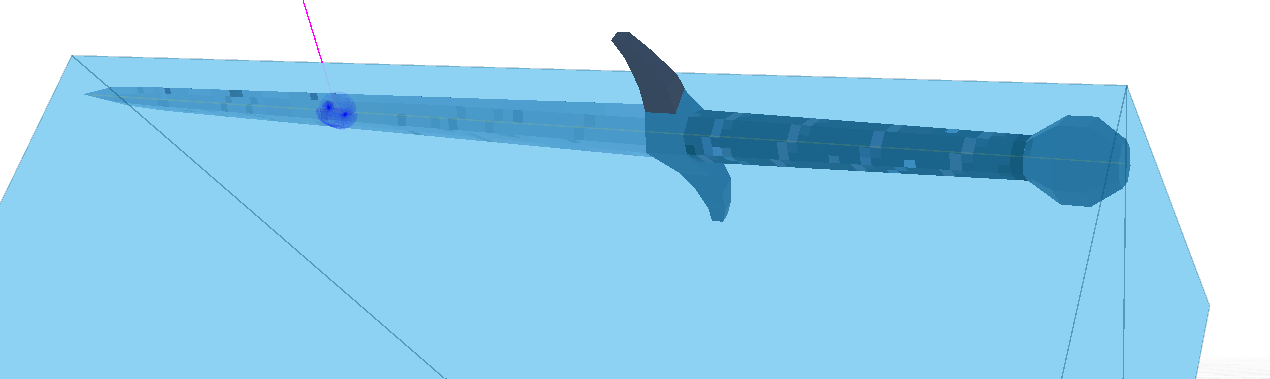
\includegraphics[width=140mm]{../img/fixerOverreach.png}
  \caption{Fixer s aktivovaným přesahem}
  \label{obr05:fixerOverreach}
\end{figure} 

\begin{figure}[ht]\centering
  \center
  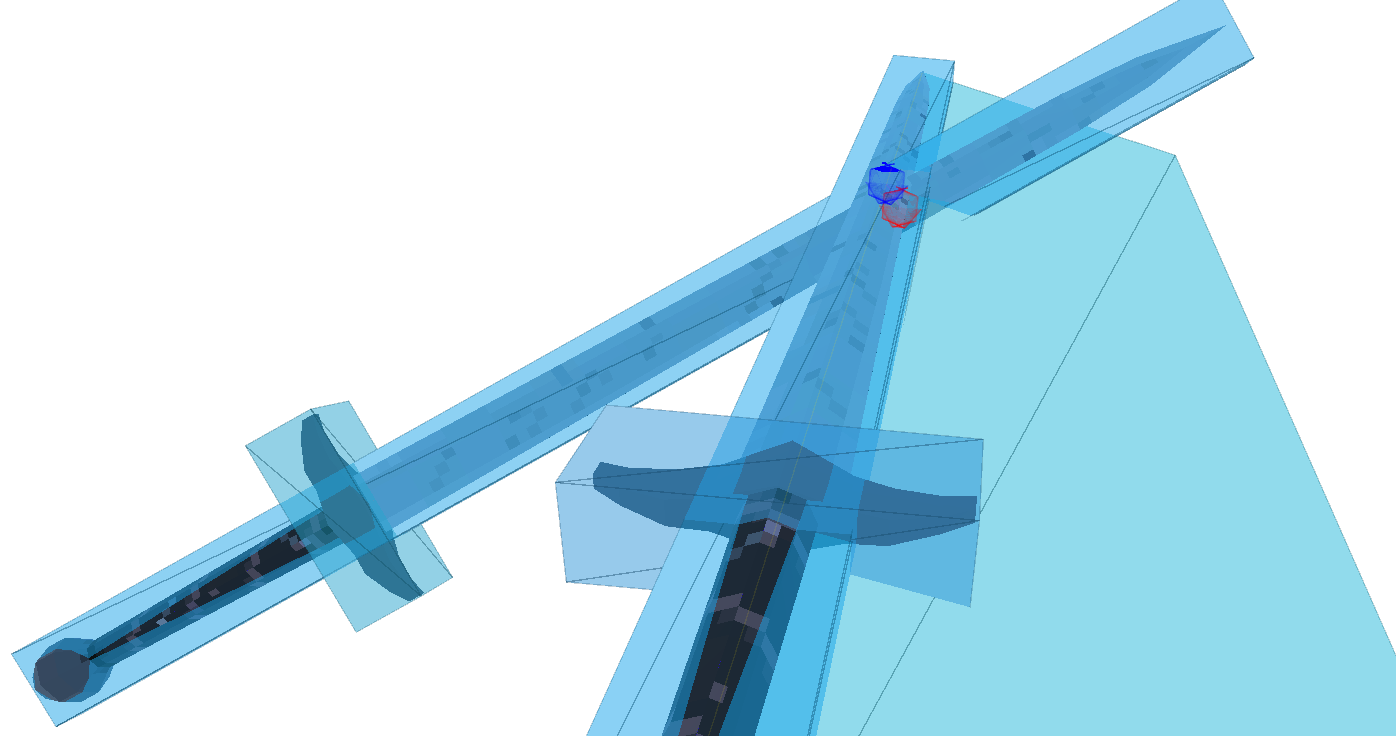
\includegraphics[width=140mm]{../img/fixerSqueak.png}
  \caption{Meč skřípnutý mezi druhý meč a jeho fixer}
  \label{obr05:fixerSqueak}
\end{figure} 



\subsubsection*{Implementace - fixer v herní scéně}

Polohování fixeru tedy je vyřešené, zbývá rozhodnout, jak jej spárujeme s Hostitelem, aby mu byla korektně předávána kolizní síla, a také jak zařídíme, aby náš fixer nekolidoval s jinými objekty než je Cílový meč.

Řešení prvního úkolu je jednoduché - fixer zkrátka umístíme jako dítě přímo do herního objektu Hostitele. Takto budou veškeré síly vzešlé z kolizí fixeru automaticky působit na celé Rigidbody meče. Síly takto aplikuje přímo fyzikální systém, měly by tedy být realistické. 

Narazili jsme na jediný problém - přidání velkého neforemného collideru meči, zdá se, naruší balanc a nutí ho se naklánět k místu, kam je fixer zrovna natočený, svižnost pohybu meče trpí. Řešení je naštěstí jednoduché - nastavit na rigidbody Hostitele ručně hodnoty \textit{centerOfMass} a \textit{inertiaTensor} (na hodnoty ke kterým jsme se dobrali v \ref{swordParameterTweaksSection}) - ty následně fyzikální systém při vytvoření a pohybu fixeru nebude automaticky přepočítávat a balanc meče, který je ve skutečnosti definován pouze těmito dvěma hodnotami, se neodchýlí z našeho pečlivě vyladěného stavu. 

\bigbreak

Zařídit, aby fixer nekolidoval s veškerými dalšími objekty, je nepatrně těžší úkol. Elegantním řešením by bylo umístit fixer na kolizní vrstvu, která nekoliduje s ničím, a selektivně pro něj zapnout kolize pouze s collidery Cíle - zhruba takto:
\begin{code}
 UnityEngine.Physics.IgnoreCollision(fixer, Cíl, false);
\end{code}
Ačkoliv by se však z formulace v oficielní dokumentaci mohlo zdát, že toto řešení bude fungovat, opak je pravdou - tato statická funkce slouží pouze jako opt-out mechanizmus pro kolize napříč vrstvami, které jsou globálně nastavené jako vzájemně kolidující.

Bylo tedy třeba sofistikovanějšího řešení. Pro fixery jsme vytvořili oddělenou kolizní vrstvu, která koliduje pouze s vrstvou pro meče. Následně jsme ke každému fixeru přidali druhý trigger collider - tomu jsme dali velikost dostatečnou na to, aby zdetekoval kterýkoliv meč v okolí dříve, než by mělo dojít k jeho kolizi s fixerem. V jeho OnTrigger callbacku zkrátka pro každý collider, který ho aktivuje a který nepatří do Cílového meče, zavoláme 
\begin{code}
 UnityEngine.Physics.IgnoreCollision(fixer, collider, true);
\end{code}

Nyní tedy ve scéně můžeme mít najednou větší množství mečů i fixerů. Každý fixer bude kolidovat pouze se svým Cílovým mečem a ostatní objekty nebude nijak ovlivňovat.


\subsubsection*{Výsledek}

Nad plody naší práce jsme pro uživatele postavili pohodlnou fasádu - komponentu \textbf{CollisionFix}. Tu stačí přidat do herního objektu meče a zařídit, aby tam spolu s ní byla komponenta \textit{SwordDescriptor}. \textit{CollisionFix} se následně postará, aby pro jakýkoliv meč, který se objeví poblíž (to detekuje pomocí velkého trigger collideru), byl vytvořen příslušný fixer. Pro každý pár mečů je vytvořen pouze jeden fixer - který z mečů bude figurovat jako jeho Hostitel a který jako Cíl se rozhodne hodem mincí. V případě zničení komponenty \textit{CollisionFix} jsou všechny fixery, pro které figuruje jako Cíl či Hostitel, rovněž korektně zničeny.

Na komponentě \textit{CollisionFix} je možné konfigurovat parametry, jež budou pro její fixery použity - hloubku, přesah, maximální vzdálenost detekce tunelování apod. - defaultní hodnoty by však měly poskytovat dobrou funkčnost. 

Vzhledem k tomu, že počet fixerů ve scéně roste v nejhorším případě kvadraticky s počtem mečů (viz obr. \ref{obr05:collisionFixGroup}), poskytli jsme uživateli prostředky k regulaci jejich vytváření - lze upravit maximální vzdálenost od meče, ve které fixery budou vytvářeny, a specifikovat objektové hierarchie, jejichž meče má \textit{CollisionFix} zcela ignorovat (např. spolubojovníci typicky nepotřebují mít vzájemné kolize ošetřené).

\begin{figure}[ht]\centering
  \center
  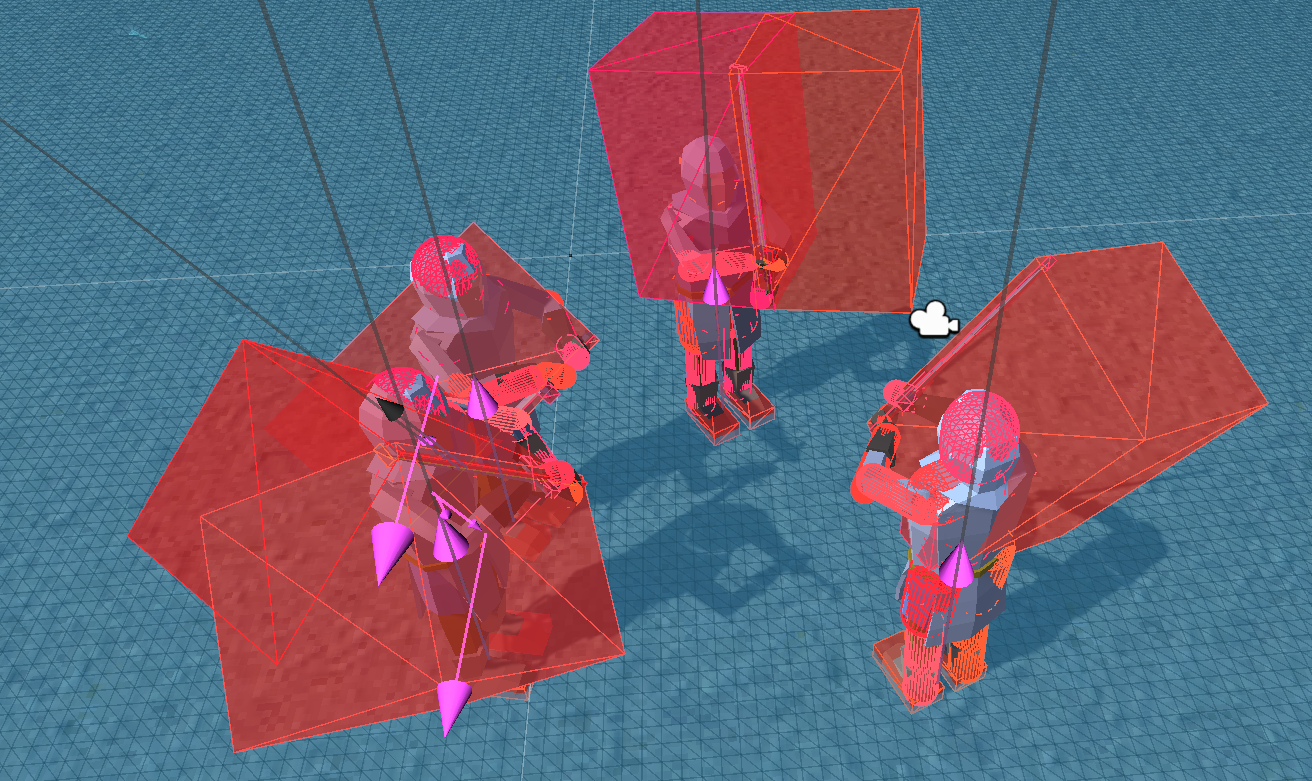
\includegraphics[width=140mm]{../img/collisionFix-group.png}
  \caption{Čtveřice šermířů s plnou vzájemnou korekcí kolizí mečů}
  \label{obr05:collisionFixGroup}
\end{figure} 


%------------------------------------------------------------------------------------------------------------------------------------------------------------------------------------------------------------------------------------------------------------%
 % xxxxxxxxxxxxxxxxxxxxxxxxxxxxxxxxxxxxxxxxxxxxxxxxxxxxxxxxxxxxxxxxxxxxxxxxxxxxxxxxxxxxxxxxxxxxxxxxxxxxxxxxxxxxxxxxxxxxxxxxxxxxxxxxxxxxxxxxxxxxxxxxxxxxxxxxxxxxxxxxxxxxxxxxxxxxxxxxxxxxxxxxxxxxxxxxxxxxxxxxxxxxxxxxxxxxxxxxxxxxxxxxxxxxxxxxxxxxxxxxxxxxxxxx %
%------------------------------------------------------------------------------------------------------------------------------------------------------------------------------------------------------------------------------------------------------------%



\section{Demo hra}

Pro demonstraci funkčnosti našeho systému jsme vytvořili drobnou akční hru, její spustitelné sestavení pro platformy Windows a Linux nalezne čtenář v příloze.

Hráčem ovládaný šermíř s mečem, kterého jsme navrhli a implementovali v předchozí části této práce, se zde může pohybovat po středověkem inspirovaném fantasy světě sestávajícím z arény obklopené lesem. V aréně může zápasit s jednoduchými počítačem řízenými protivníky.  

Než přistoupíme k bližšímu představení jednotlivých částí hry, zmiňme, že veškeré grafické assety (3D modely a textury), které jsme použili, byly vytvořeny autorem této práce a vztahuje se na ně stejná opensource licence jako na zbytek práce.


\subsection{Herní svět}

Ústředním bodem herního světa je aréna - v té se odehrává veškerý gameplay. Okolní kopcovitá krajina s rozmístěnými stromy pak slouží jako kulisy.

K vytvoření krajiny jsme použili vestavěný editor terénu, který engine Unity nabízí. Jeho pomocí jsme i rozmístili stromy - těm jsme v zájmu výkonu nepřidělili collidery, jsou čistě vizuální. Záměrem bylo pouze pro arénu vytvořit tématické a nerozptylující okolí.

Aréna je ohraničena kolem dokola palisádou. Najdeme v ní kruhové bojiště, ve kterém se spawnují nepřátelé a mají povoleno se po něm pohybovat, a malé prostranství s tlačítky, jež může šermíř stisknout svým mečem, aby spawn nepřátel inicioval - viz obr. \ref{obr05:demogameArenaLayout} 
\begin{figure}[ht]\centering
  \center
  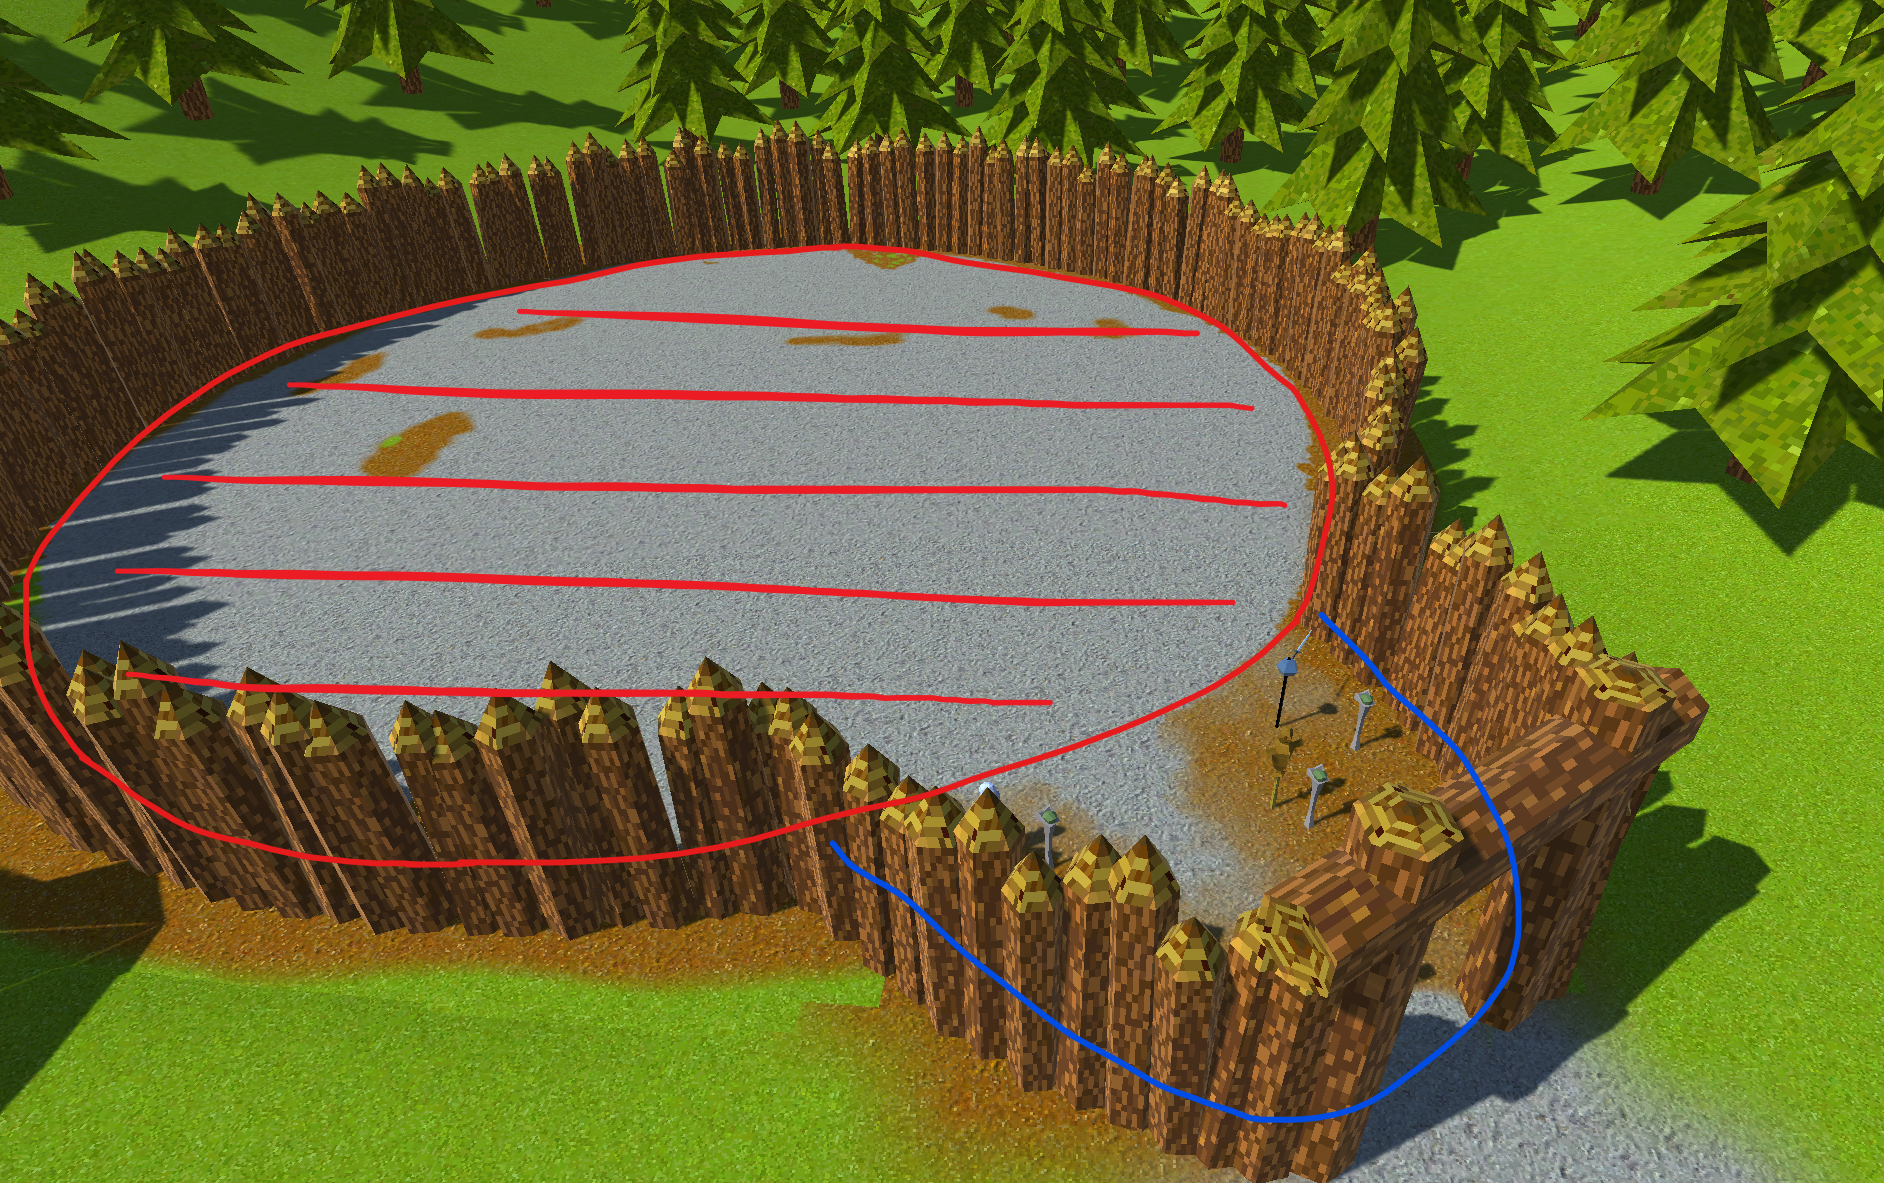
\includegraphics[width=145mm]{../img/demogameArenaLayout.png}
  \caption{Aréna - bojiště (červeně), prostranství s tlačítky (modře)}
  \label{obr05:demogameArenaLayout}
\end{figure} 

Tlačítka jsou implementována jako \textit{Damageable} s nekonečným množstvím \acs{HP}, jejichž OnDamaged event spustí kosmetický efekt probliknutí a na náhodném místě arény vykoná spawn jejich přiřazené nepřátelské entity - viz obr. \ref{obr05:demogameActivateButton}. 
\begin{figure}[h!]\centering
  \center
  \includegraphics[width=140mm]{../img/demogameActivateButton.png}
  \caption{Tlačítko stisknuté mečem a nově spawnutý nepřátelský šermíř}
  \label{obr05:demogameActivateButton}
\end{figure} 

Pro hráčovu orientaci jsme vedle každého tlačítka postavili jako ''maskota'' jednu instanci entity, kterou spawnuje - upravenou, aby stála na místě a nemohla hráče nijak zranit ani hráč ji.

Typy nepřátel jsou tři - nepřátelský šermíř, trénovací panák, třetího jsme pracovně nazvali ''mečotoč'' - podrobně je rozebereme v jejich vlastních sekcích.


\subsection{GUI}

Grafické uživatelské rozhraní jsme vytvořili pomocí vestavěného systému Unity UI, který nám umožnil jednotlivé prvky definovat skrze obyčejné objekty v hierarchii herní scény. S textovými prvky pomohl dodatečný balíček TextMesh Pro \cite{TextMeshPro}.
\bigbreak

Klávesou Escape aktivované \textbf{menu} nabízí obvyklé základní položky: restart hry, konec hry a přehled mapování kláves.
Pozastavení hry, když je hráč v menu, jsme implementovali nastavením \textit{UnityEngine.Time.timeScale = 0}.
\bigbreak

Dále zde najdeme překryvné rozhraní, jehož úkolem je hráčovi komunikovat \textbf{stav jeho postavy}. 

V levého spodním rohu najdeme healthbar - ten ukazuje jaká část z maximálního hráčova zdraví ještě zbývá. Informaci získává posloucháním OnUpdate eventu na hráčově \textit{Damageable}, který zaregistruje hráčova \textit{SwordAssembly}. Stejným způsobem na hráčovi poslouchá i druhá pomocná komponenta - jejím úkolem je na několik sekund přes obrazovku zobrazit obrázek krvavých skvrn, pokud bylo hráčovi uštědřeno obzvláště těžké zranění. Pokud hráč zemře, zobrazí se krvavé skvrny trvale spolu s výzvou, aby ''stiskl 'R' pro restart hry''.

Pro komunikaci zdraví nepřátel nepoužíváme překryvné GUI. Původní myšlenka byla nad základní texturou nepřítele postupně odkrývat druhou vrstvu s krvavými skvrnami, nakonec jsme se omezili na postupné obarvování celého nepřítele na červeno (skrze \textit{Renderer.material.color}) dle jeho zbývajících HP. Abychom ke zraněním poskytli okamžitou zpětnou vazbu, rovněž jsme zapojili \href{https://docs.unity3d.com/2022.2/Documentation/Manual/Built-inParticleSystem.html}{vestavěný Particle systém enginu Unity}, s jehož pomocí v místě zásahu emitujeme několik částic ''stříkající krve'' - viz obr. \ref{obr05:demogameEnemyBloodied}

\begin{figure}[!h]\centering
  \center
  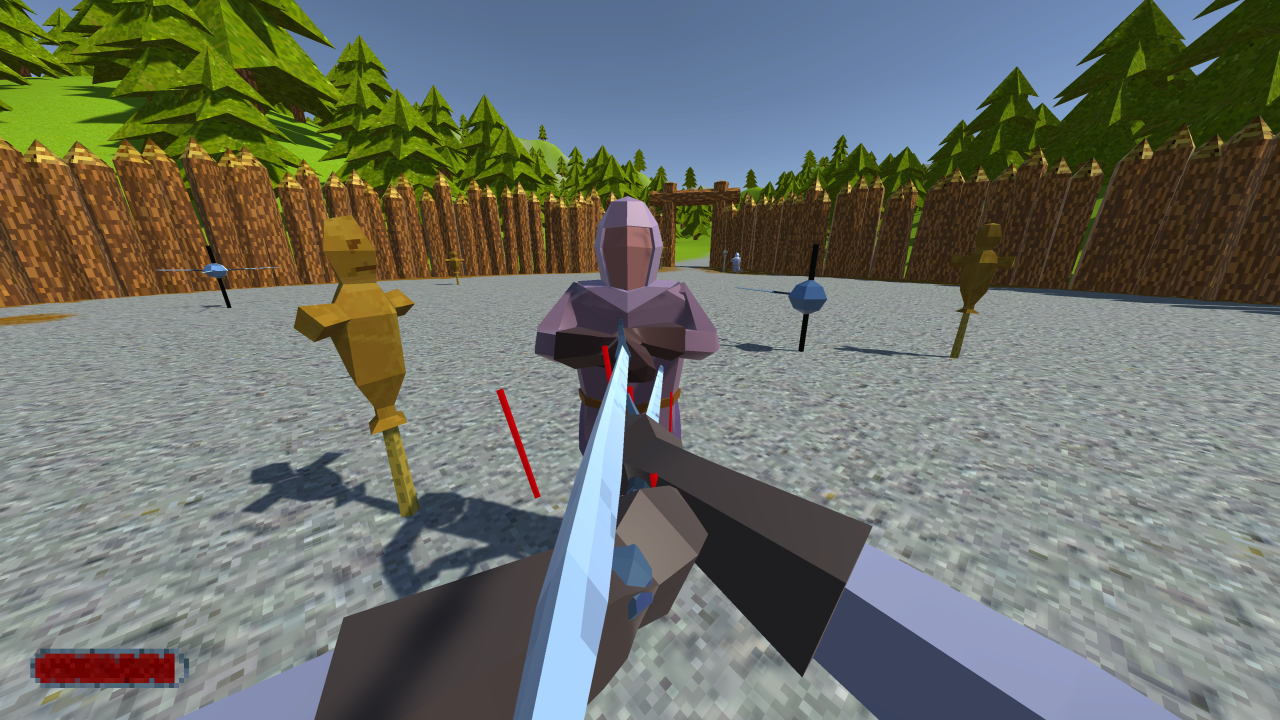
\includegraphics[width=140mm]{../img/demogameFightEnemyBloodied.png}
  \caption{Boj s mírně zraněným protivníkem}
  \label{obr05:demogameEnemyBloodied}
\end{figure} 

\subsection{Statičtí nepřátelé}

Do hry jsme implementovali dva jednodušší typy nepřátel, kteří se nemohou pohybovat po aréně a mají velmi jednoduché chování, mohou však hráči být nápomocni k testování některých herních konceptů nebo k ozvláštnění boje s nepřátelským šermířem.

\begin{figure}[h!]\centering
  \center
  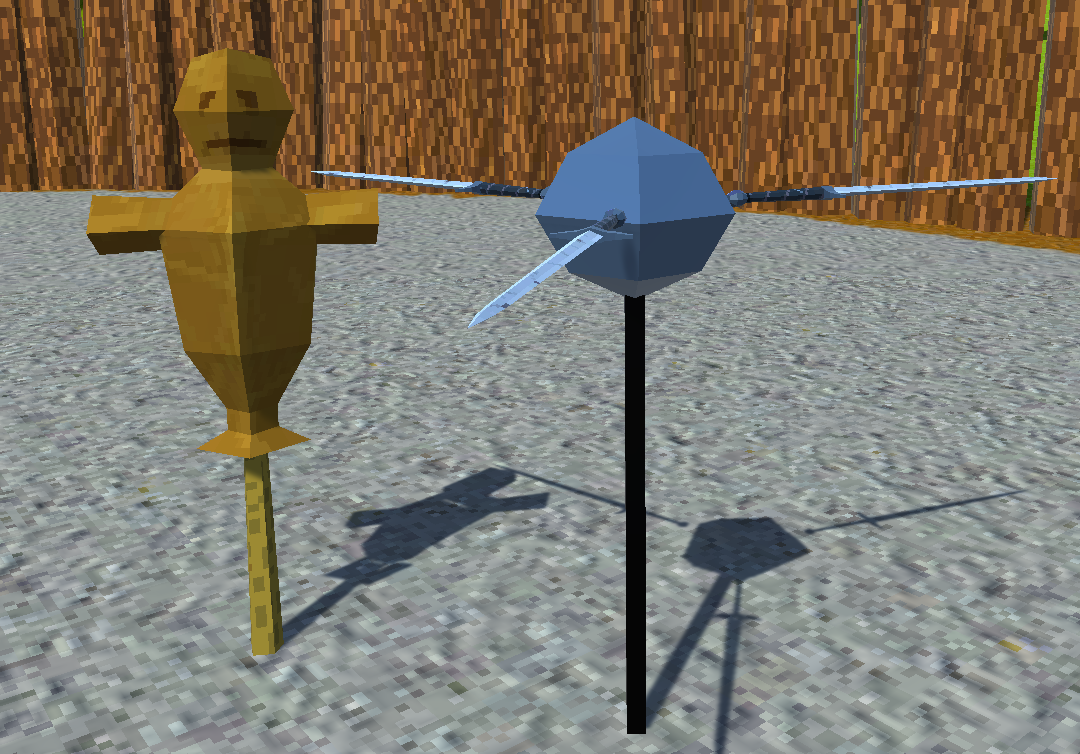
\includegraphics[width=110mm]{../img/demogameStaticEnemies.png}
  \caption{Statičtí nepřátelé - panák (vlevo) a mečotoč (vpravo)}
  \label{obr05:demogameStaticEnemies}
\end{figure} 


\subsubsection*{Trénovací panák}

Stojí na místě dokud není zničen, hráče nemůže nijak zranit. Poskytuje bezpečné prostředí, kde si hráč může vyzkoušet základní ovládání meče. 

Viz obr. \ref{obr05:demogameStaticEnemies} - vlevo.

\subsubsection*{Mečotoč}

Koule rotující na tyči zapíchnuté v zemi, ke které je připevněných několik (1 až 6) mečů. Meče mohou zraňovat ostatní entity a proti hráči\footnote{Proti ostatním mečotočům a nepřátelským šermířům jsme ji v zájmu výkonu vypnuli.} mají aktivovanou korekci kolizí (viz \ref{swordCollisionsSection}). Hráči může posloužit ke cviku blokování a podobných pokročilejších technik. Mečotoč, kterému byl při spawnu vylosován větší počet mečů a agresivní pattern pohybu, může sám znamenat zajímavou herní výzvu srovnatelně obtížnou jako nepřátelský šermíř. 

Koule je ke středové tyči připojena pomocí \textit{ConfigurableJointu} a rotována nastavením nenulové položky \textit{joint.targetAngularVelocity}. Vytvoření, rozmístění a připojení stanoveného počtu mečů jointem ke kouli vykonává při spawnu komponenta \textit{SwordmillAssembly}. Nakonec jsme pro ozváštnění přidali i schopnost koule posunovat se po tyči nahoru a dolů podle náhodně definovaného patternu - to je starostí komponenty \textit{SwordmillBehavior}.

\subsubsection*{Randomizace}

Pro randomizaci nepřátel jsme stanovili rozhraní \textit{IRandomizer} - to má jedinou metodu \textit{Randomize()}, která bere jako parametr instanci \textit{System.Random}. Spawnovací mechanismus na každé entitě při spawnu projde všechny komponenty v její hierarchii, které toto rozhraní implementují, a metodu \textit{Randomize()} na nich zavolá.

Na mečotoči i na trénovacím panákovi např. používáme \textit{TransformRandomizer} - ten podle stanovených parametrů náhodně pozmění polohu, rotaci a velikost objektu.

Pro mečotoč největší pozornost zasluhuje \textit{SwordmillRandomizer} - ten randomizuje počet mečů, cestu koule nahoru/dolů po tyči a rovněž sílu, s kterou jsou meče koulí drženy.


\subsection{Počítačem řízený šermíř} \label{knightEnemySubsection}

Při tvorbě nepřátelského šermíře jsme se snažili využít co nejvíce již existujících komponent vyvinutých pro hráčského šermíře. Výsledek tomu odpovídá - k původnímu prefabu hráčského šermíře nám stačilo až na několik detailů pouze přidat algoritmus strojové inteligence a vyměnit zdroj vstupu za simulovaný, který má algoritmus pod kontrolou. Rovněž bylo samozřejmě třeba zpřetrhat veškeré vazby na herní kameru a GUI - objekty, které náleží pouze hráči.

Algoritmus umělé inteligence implementuje komponenta \textit{SwordsmanAI} - tu jsme přidali do kořenového objektu spolu s komponentou \textit{InputSimulator}, kterou jsme nahradili za původní \textit{BasicSwordInput}. Do jeho pole Cíl jsme v editoru přetáhli hráčského šermíře.


\subsubsection*{Pohyb po terénu}

Nejprve se zaměřme na šermířův pohyb po aréně. Především chceme, aby šermíř pronásledoval hráče, ale bylo by příhodné, kdyby se při tom dokázal vyhýbat ostatním šermířům a statickým nepřátelům, kteří jsou po aréně rozmístění. Přesně to je úkol, který řeší standardní knihovna \textbf{NavMesh} (více se o ní čtenář dozví v \href{https://docs.unity3d.com/2022.2/Documentation/Manual/Navigation.html}{oficielní dokumentaci} \cite{Unity}).

Uvnitř arény jsme tedy vytvořili \textit{NavMeshSurface} (objekt definující terén po kterém je možné se pohybovat) a statickým nepřátelům jsme přidali komponentu \textit{NavMeshObstacle}. Zbývá pouze šermířovi přidat komponentu \textit{NavMeshAgent}.

\textit{NavMeshAgent} si pro účely navigace vede vlastní reprezentaci postavy, která se pohybuje nezávisle od jejího fyzického těla. Defaultně po každém updatu updatuje i transform postavy, aby interní reprezentaci odpovídal, my však chceme postavou pohybovat ručně manipulací jejího \textit{ISwordInput}. K tomu bylo třeba vypnout flagy \textit{agent.updatePosition}, \textit{agent.updateRotation} a \textit{agent.updateUpAxis}. 

Každý snímek na agentovi zavoláme metodu \textit{agent.SetDestination()}, které předáme aktuální pozici hráčského šermíře, a následně našeho šermíře pohneme směrem k interní pozici agenta:
\begin{code}
 agent.SetDestination(TargetSwordsman.transform.position);

 var direction = agent.nextPosition - this.transform.position;
 var forward = direction.DotProduct(this.transform.forward); 
 var right = direction.DotProduct(this.transform.right);
 
 inputSimulator.SetAxis(InputMapping.Forward, forward * ForwardSpeed);
 inputSimulator.SetAxis(InputMapping.Sideways, right * SidewaysSpeed);
\end{code}
Pro horizontální rotaci šermíře se osvědčilo použít stejnou hodnotu jako pro pohyb bokem:
\begin{code}
 inputSimulator.SetAxis(InputMapping.RotateHorizontal, 
                        right * RotateHorizontalSpeed)
\end{code}
Aby se nehromadil rozpor mezi pozicí agenta a skutečnou pozicí šermíře, je třeba nakonec agenta k šermířovi přiblížit zpátky - oficielní dokumentace doporučuje takto:
\begin{code}
 agent.nextPosition = this.transform.position + 0.9 * direction;
\end{code} 

Nyní je šermíř schopen se pohybovat po aréně, pronásledovat hráče a při tom se vyhýbat překážkám i dalším šermířům - viz obr.\ref{obr05:demogameAiNavigation}.

\begin{figure}[h!]\centering
  \center
  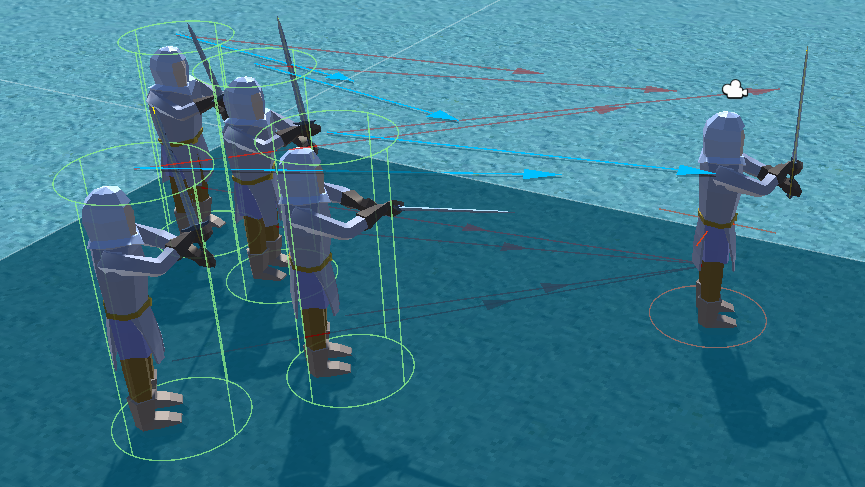
\includegraphics[width=120mm]{../img/demogameAiNavigation.png}
  \caption{Skupina šermířů koordinovaně pronásledující hráče (zelený válec značí interní NavMeshAgent polohu)}
  \label{obr05:demogameAiNavigation}
\end{figure} 


\subsubsection*{Ovládání meče}

Pro tvorbu nahrávek pohybů meče jsme měli dvě možnosti:
\begin{itemize}
  \item Nahrávat uživatelský vstup
  \item Nahrávat volání \textit{SwordMovement.MoveSword()}
\end{itemize}

Zvolili jsme druhou možnost, protože takto pořízené nahrávky mohou fungovat spolehlivě nezávisle na aktuální konfiguraci \textit{SwordMovement.Modules}, které na šermířském prefabu chceme v budoucnu dále ladit a měnit. Rovněž se systémem, který k takovémuto účelu vytvoříme, by později nemělo být obtížné např. zavést přehrávání nahrávek i jako dodatečný mod ovládání pro hráčského šermíře, podobně jako to umožňuje hra \acl{DbtS} (viz \ref{dieByTheSwordDescriptionSubsection}).

\bigbreak

Nejprve bylo tedy třeba \textbf{pořídit nahrávky}. K tomuto účelu jsme vytvořili komponentu \textit{SwordMovementRecorder} - ta při vytvoření vměstná mezi SwordMovement a jeho moduly dekorátor (jako jsme si nastínili v \ref{implementationSwordSubmodulesSubsubsection}), který zachytává volání \textit{MoveSword()} a reportuje je callbackem nahrávací komponentě. Komponenta následně reportované instrukce pro pohyb meče převede do souřadnic relativních vůči Transformu šermíře a opatří timestampem. Sekvence takových instrukcí je nakonec uložena na disk jako textový soubor ve formátu JSON (k tomu jsme použili knihovnu Newtonsoft.Json \cite{NewtonsoftJson}).

\bigbreak

Výsledný list souborů s nahrávkami následně v editoru přiřadíme do příslušného pole komponenty \textit{SwordsmanAI}. Ta je při své inicializaci deserializuje a následně v komponentě \textit{SwordMovement} násilně vymění list modulů za vlastní - s jediným defaultním modulem \textit{PlayRecord}. Ten jednotlivé snímky nahrávky postupně předává metodě \textit{MoveSword()}. Orientuje se při tom podle timestampů a herního času, bylo tedy jednoduché přidat násobič, kterým lze přehrávání zrychlit či zpomalit.

Nahrávky jsme rozdělili do dvou skupin - útok a idle - útok se zapne, když je šermíř nablízko svému cíli, jinak se přehrává idle. Přehrává se jedna náhodně vybraná nahrávka z aktivní skupiny.

\subsubsection*{Shrnutí}

Podařilo se nám vytvořit nepřítele, který je schopen po aréně pronásledovat hráče a útočit na něj přehráváním předpřipravených útoků. Drtivou většinu herní logiky jeho implementace sdílí s hráčskou postavou.

\begin{figure}[h!]\centering
  \center
  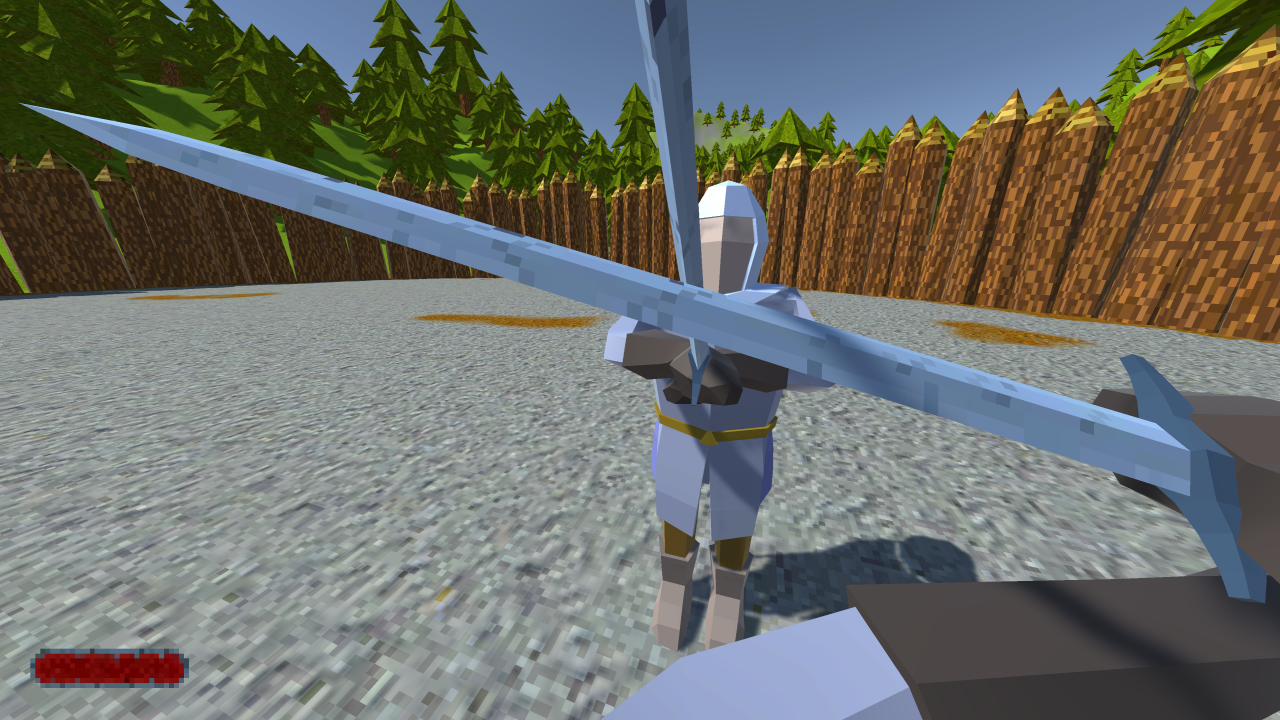
\includegraphics[width=140mm]{../img/demogameFight.png}
  \caption{Šermíř útočící na hráče}
  \label{obr05:demogameFight}
\end{figure} 

\section{Shrnutí}

Dokončili jsme implementaci naší práce. Meč i šermíř jsou plnohodnotnými prvky fyzikální simulace se všemi výhodami, které toto přináší např. pro možnosti interakce s okolním prostředím. Pro meč jsme implementovali dva základní submoduly ovládání - sekání a blokování. Pro tělo šermíře jsme vytvořili za použití standardního balíčku Animation Rigging \cite{AnimationRigging} procedurální animaci, která zajišťuje, že kosmeticky ''drží'' meč. Rovněž jsme načrtli systém životů a výpočtu zranění.

Velkou výzvou bylo zajistit realistické \textbf{chování mečů při kolizích}. Žádná z metod detekce kolizí, které Unity nabízí, nebyla schopna zcela zabránit tunelování. Řešením bylo pro každý pár mečů vytvořit dodatečný ''velký'' collider, který se nacházel na jednom z mečů a natáčel se dle polohy toho druhého. Dalším netriviálním úkolem bylo vyladit fyzikální parametry, aby bylo dosaženo plynulého pocitu při švihu mečem. 

Pro praktickou demonstraci možností našeho systému jsme následně vytvořili ukázkovou hru. Hráč zde může v prostředí fantasy arény zápasit s jednoduchými počítačem řízenými protivníky, kteří používají standardní systém NavMesh pro orientaci v terénu a útočí přehráváním přednahraných pohybů meče. 
